\documentclass[conference]{IEEEtran}
\IEEEoverridecommandlockouts
% The preceding line is only needed to identify funding in the first footnote. If that is unneeded, please comment it out.
\usepackage{cite}
\usepackage{amsmath,amssymb,amsfonts}
\usepackage{algorithmic}
\usepackage{graphicx}
\usepackage{textcomp}
\usepackage{xcolor}
\usepackage{tabularx,booktabs}
\usepackage{longtable}
\usepackage{enumitem}
\usepackage{placeins}
\usepackage{kotex}
\newcommand\custompicheight{25em}

\def\BibTeX{{\rm B\kern-.05em{\sc i\kern-.025em b}\kern-.08em
    T\kern-.1667em\lower.7ex\hbox{E}\kern-.125emX}}
\begin{document}

\title{Before Order - A menu information providing chatbot service}

\author{\IEEEauthorblockN{1\textsuperscript{st} Kang Minju}
\IEEEauthorblockA{\textit{dept. Information System} \\
\textit{Hanyang Univ.}\\
Seoul, South Korea \\
kmj1997@gmail.com}
\and
\IEEEauthorblockN{2\textsuperscript{nd} Lim Hyojin}
\IEEEauthorblockA{\textit{dept. Information System} \\
\textit{Hanyang Univ.}\\
Seoul, South Korea \\
hyojin12288@gmail.com}
\and
\IEEEauthorblockN{3\textsuperscript{rd} Choo Yedeun}
\IEEEauthorblockA{\textit{dept. Information System} \\
\textit{Hanyang Univ.}\\
Seoul, South Korea \\
cydddd1221@gmail.com}
\and
\IEEEauthorblockN{4\textsuperscript{th} Christian Gärtner}
\IEEEauthorblockA{\textit{dept. Computer Science} \\
\textit{Hanyang Univ.}\\
Esslingen am Neckar, Germany \\
christian.gaertner97@gmail.com}
}

\maketitle

\begin{abstract}
Globalization attracted many newcomers to South Korea but our restaurant services have not kept up with the needs of foreign customers. Foreigners still have difficulties reading and understanding menus in traditional but also modern Korean restaurants. Therefore, we will develop ‘BeforeOrder’ by using the ‘Facebook Messenger’ chatbot API and provide foreigners with a service to conveniently receive information about menus and dishes throughout their journey.
\end{abstract}

\begin{IEEEkeywords}
translator, chatbot
\end{IEEEkeywords}

\section{Introduction}
Many foreigners are often lost and embarrassed when eating out at restaurants as they can neither read the foreign menus nor can they understand what ingredients are used for specific dishes. Those things can make it hard to try and enjoy foreign food especially for people who have allergies and therefore have to ask the staff every time. But staff members, especially in more rural areas, often do not speak or understand English and cannot provide sufficient information. On the other hand, restaurants often simply do not have the space in menus to list the name of dishes and its ingredients in both, the foreign and the English language.

 Whenever foreigners face this situation, they have to search and retrieve all the different information manually. However, foreigners who do not know ‘Hangeul’ will not be able to search directly on Google because they do not understand the dish names in a menu and often also do not have access to a ‘Hangeul’ keyboard. Even if someone searches for the information, it may not be properly categorized and recognized by a translator as they often do not distinguish dishes and it may happen that they simply translate the individual letters into English. Eventually the user may need to search more and more and ends up leaving the restaurant and eat someplace else. 

 We will try to solve this problem with ‘KakaoTalk’, a chat application that is essential in Korea. Since 2013, Kakao has provided an automated response API through KakaoTalk Plus Friends. Plus Friends can be added as a friend in KakaoTalk to receive various contents, benefits and information. Using this method, the user can conveniently install and delete the service provided by us and also use the functionality with an intensively tested and user-friendly interface.

 A chatbot in general describes an artificial intelligence-based program, that analyzes the conversation with a user. Users of the messenger can naturally send messages or ask questions to a chatbot which in return provides a service that responds to the user and seems to communicate with him. There are multiple reasons as to why KakaoTalk chatbots are getting attention. First, it has a familiar UX design and developing a new UX can be very time-consuming and users may have difficulties adapting to a new design. Second, people tend to be reluctant to download new apps for a variety of reasons. Third, using a popular and well-known messenger improves accessibility. We think using a chatbot will increase the popularity of the service and make it more appealing to customers in our target audience. 

 [Before Order] target customers are foreigners that are not familiar with the Korean language and alphabet and therefor having problems eating out. The service is especially aimed at exchange students and employees who plan to stay in Korea in the long term instead of tourists that will mostly eat in international restaurants. [Before Order] follow this process: 
\begin{enumerate}
\item befriend [Before Order] as a Plus Friend in KakaoTalk
\item provide information about the menu to the chat bot in form of images or text
\item receive information about a dish by choosing from the menu list provided by [Before Order]
\end{enumerate}
That way, customers can 
\begin{itemize}
\item reach the service anytime
\item receive information about dishes without searching multiple times
\item do not have to register up for any service except befriending [Before Order] on KakaoTalk
\end{itemize}

\begin{table}
\caption{User Roles}
\begin{tabularx}{\linewidth}{|X|X|X|}
\toprule
Role                & Name              & Task and description \\
\midrule
User                & Choo Yedeun       & Assumes user point of view and guarantee a usable and user-friendly software \\
Customer            & Lim Hyojin        & Provides detailed software requirements and reviews delivered features \\
Software Developer  & Christian Gärtner & Responsible for writing and developing software features and satisfying the needs of the costumer    \\
Development Manager & Kang Minju        & Supervises the development of the service, managing of deadlines and evaluation of software features
\end{tabularx}
\end{table}
\section{Requirements}
\subsection{Functional requirements}The system will be usable on a smartphone – In order to enable the user to use the provided service while the user is moving around the system has to be reachable from a mobile platform. The user also shall be able to conveniently use a camera to take pictures of the menu without having to type and search for one dish name at a time.
The system should be usable on notebooks, tablets and stationary computers – The user shall be able to use the service at home or similar environments to be able to gather information about restaurants and dishes and help with the selection of a place to eat.
The system will run on Android, iOS and Windows 7/8/10 – The system shall run on the most popular operation systems in order to be accessible for as many users in the target audience as possible.
The system will run within a common third-party software – The user shall be provided with an intensively tested and user-friendly interface. In addition, the user should not have to download a separate application to use the functionalities of this system but instead use this service as an extension to a familiar and popular application.
The system shall provide contact information to enable the user to contact the support – The user shall be able to receive help in case of questions or problems with the service. In addition, the user should be able to report any bugs that he finds while using the service or give feedback about it.
The user shall be able to save information about a dish – The user should be able to retrieve information about dishes that he once searched for without having to query the search again. The user should also be able to read the information after closing and reopening the application.
The system shall support the Korean alphabet as input
The system will display information about dishes in the English language and alphabet
The user shall be able to select a dish in the analyzed menu and receive detailed information for this specific dish
The system should provide information about the dishes in form of used ingredients, possible allergies and level of spiciness
The system shall accept pictures and text as input – The user should be able to manually search for a dish if the analyzing of the picture returns no matches
The system should distinguish between dish names and random letter clusters – The user may input pictures without a menu or the pictures that include random text in addition to the menu

\subsection{Working mechanisms}
1. Register service
User will search for [Before Order] in the KakaoTalk Plus Friend list and add the chatbot as a friend. Registration process is finished.
2. Input information
Take a picture of a menu written in Korean alphabet and send it to the [Before Order] chat bot.
3. Recognition process
The [Before Order] service analyzes the input picture or text and tries to recognize the dishes.
4. Select information
If the user sent a whole menu he can select a single dish out of the list that [Before Order] provides and receive more detailed information for that specific dish.
5. Display detailed information
[Before Order] provides the user with detailed information about the requested dish using public APIs.

\section{Development Environment}
\subsection{Choice of software development platform}
\begin{table}[htb]
\caption{Development Tools}
\begin{tabularx}{\linewidth}{|X|X|}
\toprule
Tool & Usage \\
\midrule
Python & We’ve chosen Python as a overall basic language in developing \emph{Before Order} Python language is relatively simple, easier to read, and provides a variety of libraries in the process of implementation. Also, It is a language our team members are all familiar with.\\
Github	& We decided to use Github because it provides the necessary management functions for software development including the basic functions of the Git such as bug tracking, functional requests, task management and etc. Also, we can easily share and develop program sources together with our team members.\\
Visual Studio & Visual studio is an integrated development environment(IDE) program made from Microsoft that includes many features as compiler, editor and debugging. We are going to utilize many various necessary functions of visual studio in practical implementation.\\
Slack & Slack is a collaborative tool that enables more efficient work and communication while developing software. We are going to take advantage of the work messenger functionality of slack and its convenient drag-and-drop format file sharing
\end{tabularx}
\end{table}
\FloatBarrier

\subsection{Software in use}
The similar software can be referred to as Samsung \emph{Bixby vision}. \emph{Bixby vision} automatically extracts text messages through camera lens and translate them into user-set languages in real time. In order to use \emph{Bixby vision} menu analysis, we can just bring the camera lens to the menu. However there are two major differences that suggest why our \emph{Before Order} is better than ‘Bixby vison’. First, \emph{Bixby vision} only provide literal interpretation of food name. Therefore people are more likely to have difficulties not knowing what exactly it means. However \emph{Before Order} give more clear information as it aims to provide photo, detailed explanation and name of the food/menu in english. Lastly \emph{Bixby vision} is limited to only samsung product but our \emph{Before Order} is available on all platforms and devices since it will be implemented in chat-bot.

\subsection{Cost estimation}
\begin{table}[htb]
\caption{Development Tools}
\begin{tabularx}{\linewidth}{|X|X|}
\toprule
Tool & Cost \\
\midrule
SQL database \& server & 16870.76 Won  for 5GB / 10 DTU\\
Computer Vision API & 2811.63 Won for 1000 transactions\\
\end{tabularx}
\end{table}
\FloatBarrier

The OS version in which we will develop the program is Window 10, and We will use our own laptop for developing our service.

We will also use cloud computing service using Azure cloud platform. 
The service we are using for making our service is:
\begin{enumerate}
\item SQL Database 
\item Azure server : Azure Virtual machine
\item Computer Vision API : OCR api
\end{enumerate}
We will put our bot service in the server using Azure virtual machine. In that virtual machine, we will upload our program for our bot service and Computer vision api.  
In order to store and manage the menu data, we will connect our Bot service with the SQL Database from Azure. We will make database for storing korean and english name of the menu and the details about menu (picture, ingredients, taste, spicyness, etc).
Computer vision api will provide us texts from the picture that users send through the bot.

\section{Specifications}
\subsection{Facebook Chatbot}
The service will be provided to the user by utilizing the Facebook chatbot. The following figure Fig. \ref{fig:facebook_overview} further details the general design of the system. Requests from the user will be processed by the bot using a text recognition software and our own database with information about various dishes.

\begin{figure}[htbp]
\centerline{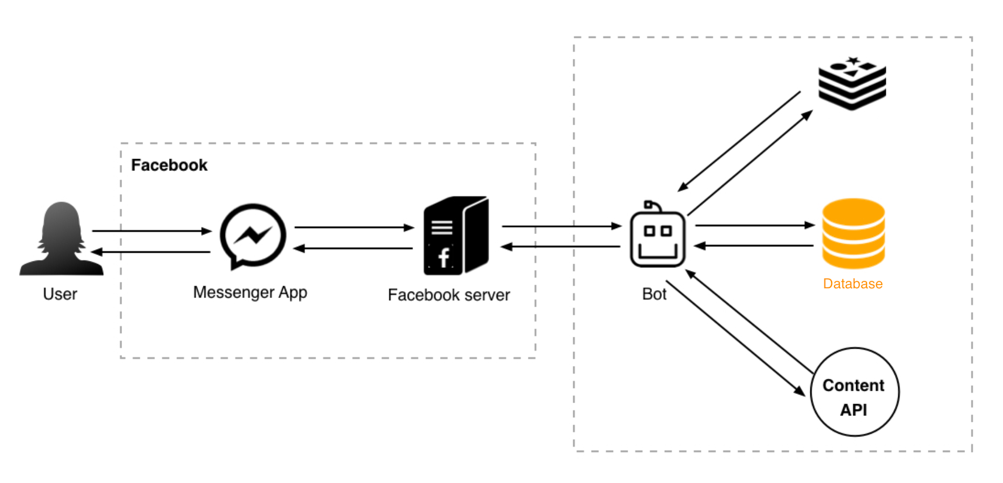
\includegraphics[width=\linewidth]{./pictures/facebook_overview}}
\caption{Overview of the system}
\label{fig:facebook_overview}
\end{figure}
\FloatBarrier

Using the Facebook Messenger as interface for our service, the user doesn't have to download a separate application and is already accustomed to navigate within the application and its usage. In order to use the service the user has to search for the \emph{Before Order} page on Facebook and send the profile a message by clicking the \emph{Send Message} button.

\begin{figure}[htbp]
\centerline{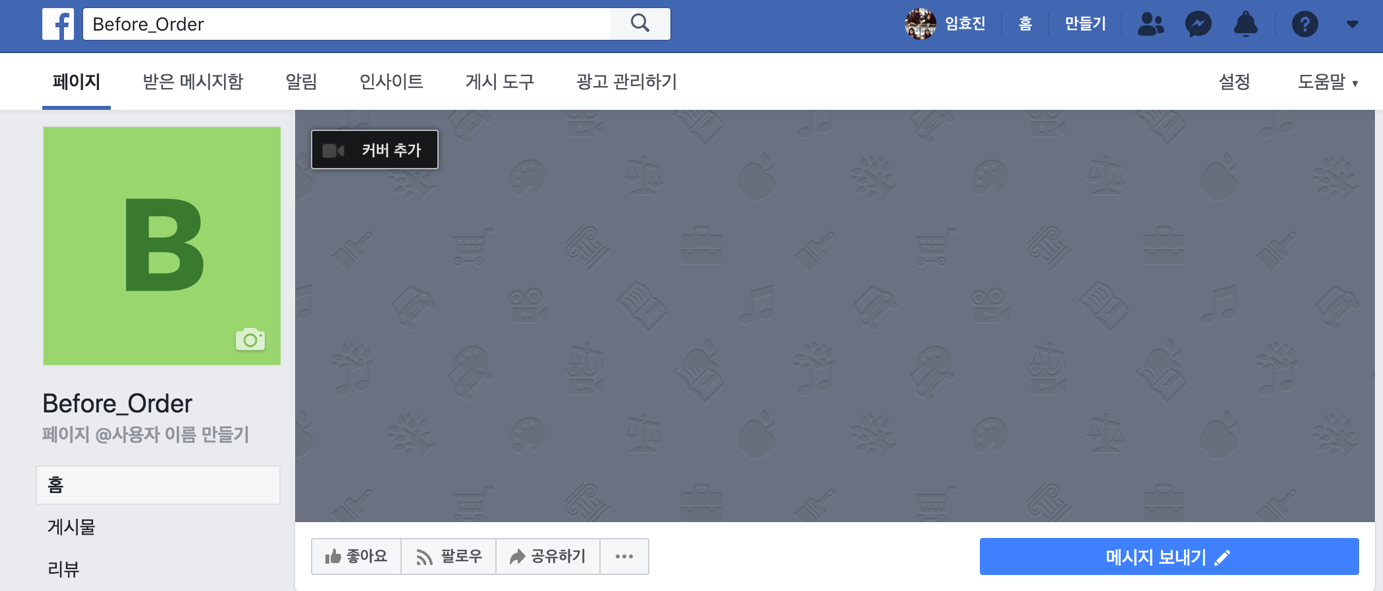
\includegraphics[width=\linewidth]{./pictures/facebook_profil}}
\caption{Chatbot profil on Facebook}
\label{fig:facebook_profil}
\end{figure}
\FloatBarrier

\subsubsection{Facebook messenger}

Given that the user has sent a message to the \emph{Before Order} service, the chat will be easily accessible from then on in the chatroom section of the Facebook Messenger application.

\begin{figure}[htbp]
\centerline{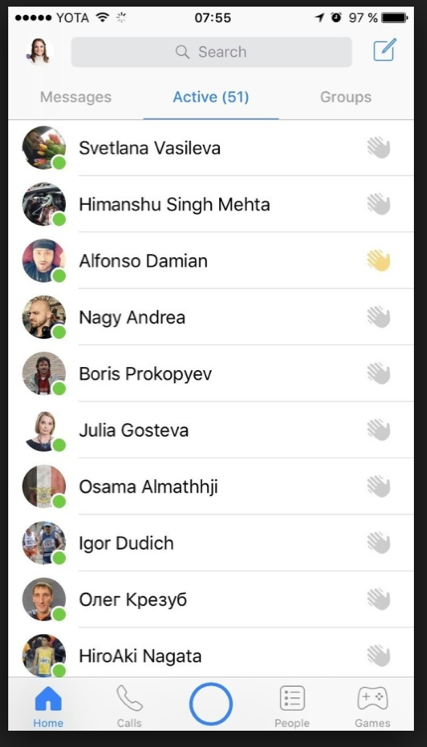
\includegraphics[height=\custompicheight]{./pictures/facebook_friends}}
\caption{Homescreen of the Facebook Messenger}
\label{fig:facebook_friends}
\end{figure}
\FloatBarrier

By selecting \emph{Before Order} from the list, the user is now able to provide a picture or dish names in the Korean alphabet to the chatbot by sending an image or a text message as shown in Fig. \ref{fig:facebook_message}

\begin{figure}[htbp]
\centerline{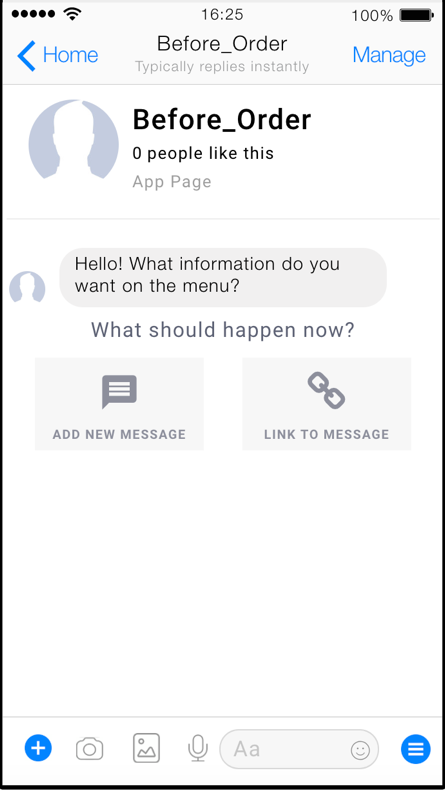
\includegraphics[height=\custompicheight]{./pictures/facebook_message}}
\caption{Chatroom with the \emph{Before Order} chatbot}
\label{fig:facebook_message}
\end{figure}
\FloatBarrier

\subsubsection{Chatbot input}

If the user sends the menu in form of a picture, the dish names have to be spelled out and need to be visible. The user can either send a picture that he took in the past or use the camera function in the Facebook Messenger to capture a picture and directly send it to the chatbot.

\begin{figure}[htbp]
\centerline{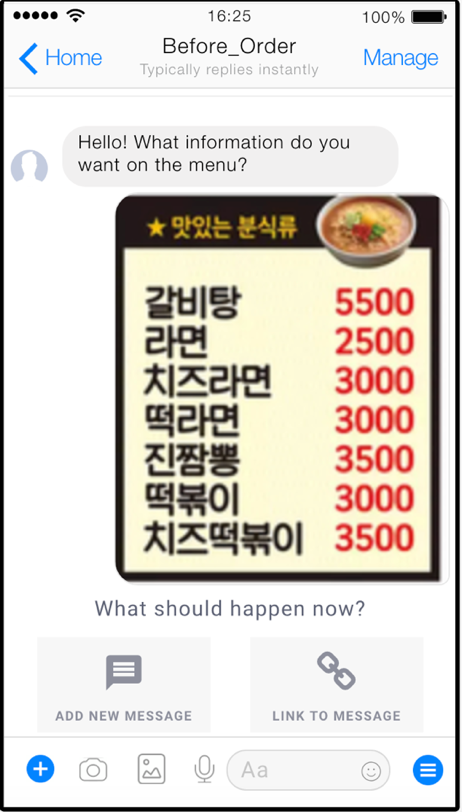
\includegraphics[height=\custompicheight]{./pictures/facebook_menu}}
\caption{Message to the chatbot including a picture of a menu}
\label{fig:facebook_menu}
\end{figure}
\FloatBarrier

Using a text recognition API and analyzing the image we are able to provide a list with all the found and supported dish names. The user is now able to select a dish that he wants more detailed information about as shown in Fig. \ref{fig:facebook_response}.

\begin{figure}[htbp]
\centerline{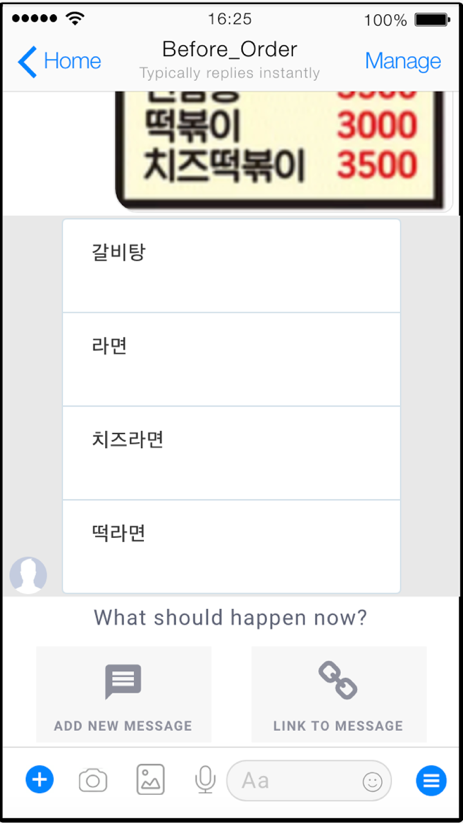
\includegraphics[height=\custompicheight]{./pictures/facebook_response}}
\caption{Response of the chatbot with all the found dishes}
\label{fig:facebook_response}
\end{figure}
\FloatBarrier

\begin{figure}[htbp]
\centerline{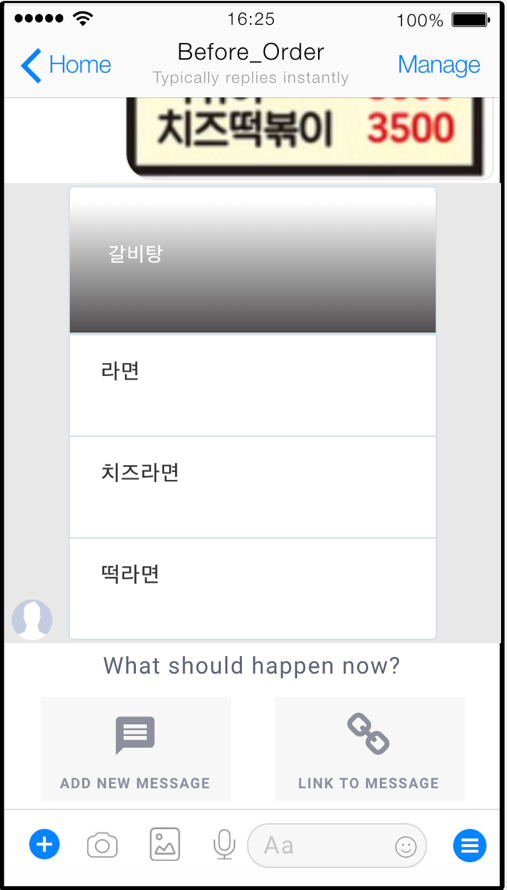
\includegraphics[height=\custompicheight]{./pictures/facebook_response_selection}}
\caption{User selecting a dish from the list}
\label{fig:facebook_response_selection}
\end{figure}
\FloatBarrier

\subsubsection{Processing of the input}

\begin{itemize}
\item Get the information from database

The information for dishes will be provided by our own database. Instead of using an open-source API for translating korean words to english we will be using an own mapping between english and korean dish names as the common translators don't support uncommon dish names or variants of dish names. Therefore each dish will have an english and an korean name associated with it to make it possible to search for dishes inside the database using korean letters. Hence most of the processes in and around the database will have to support and communicate using the UTF-8 encoding. The database will also contain a one or two sentence description for each dish, a list with its main ingredients and additional flags, such as \emph{spicy}. Managing and searching for information in this kind of database has the advantage, that:

    \begin{itemize}
    \item information for every dish is consistent and unlike as in popular search machines, such as \emph{Wikipedia} and \emph{Google}, every entry in the database will have the common information
    \item we can be sure information and names in the database refers to a dish, which enables us to filter out random textsequences and unrelated korean words and sentences
    \item we don't have to rely on the authenticity of information from a third party
    \end{itemize}

\item Server that can run chatbot and chatbot service

We will use Azure Virtual Server to run our chatbot. There are three parts in our chatbot service in the virtual machine. First one is a script that is connected with Facebook Chatbot API. This script will have scenario to answer users' requests and call other scripts to provide information to the users. Second one is to recognize the texts from the picture that users give using Computer Vision API, and the last one is for interacting with the database. When the chatbot gets the input from the users, it will call the script for text recognition. And the results will be sent again as a list format to the users. The other input that user chooses in the list will be given to the chatbot. Then chatbot will call the script for retrieving data from the database and return the detailed information about the dish to the user.

\item Vision api connection

When chatbot calls a program that is connected with Computer Vision API, It will send the picture to the Computer Vision API and get the results from it. It includes a request using the key and endpoint of the Computer Vision API. When the program sends the request to the API, it gets a result as a json format. The program also includes refine part. It refines the result text and make a result as a list format.  it returns the list-format result to the chatbot.
\end{itemize}
\FloatBarrier

\subsubsection{Chatbot output}

\begin{figure}[htbp]
\centerline{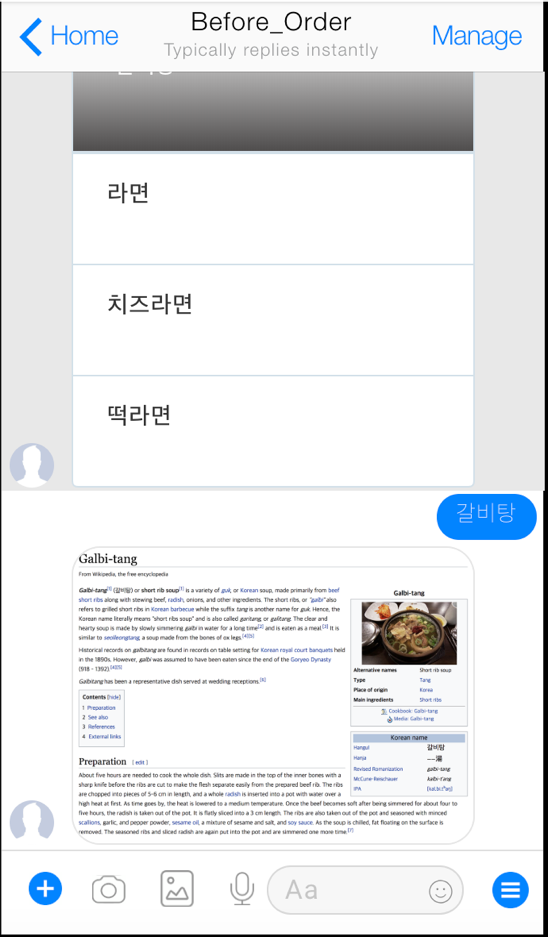
\includegraphics[height=\custompicheight]{./pictures/facebook_dish_information}}
\caption{Detailed informations about the selected dish}
\label{fig:facebook_dish_information}
\end{figure}
\FloatBarrier

Although we can not represent it in this prototype, we plan to provide information from our internal database. Users will be able to receive images of the dishes and a detailed description with ingredients.

\subsubsection{Exit}
If you need information about other menus, please feel free to send us a message.
\section{Architecture Design \& Implementation}
\subsection{Overall architecture}

\begin{figure}[htb]
\centerline{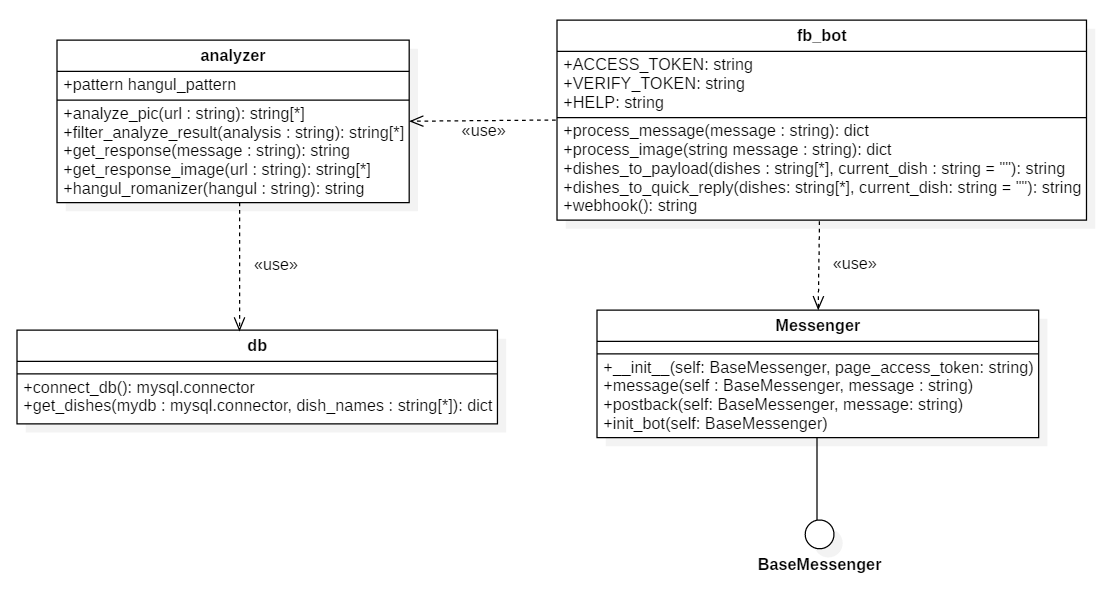
\includegraphics[width=\linewidth]{./pictures/uml}}
\caption{UML of our overall architecture}
\label{fig:uml}
\end{figure}
\FloatBarrier

\subsection{Directory organization}

\begin{table}[htbp]
\caption{Directory organization}
\begin{tabularx}{\linewidth}{|X|X|X|}
\toprule
Directory & File names & Module names in use  \\
\midrule
./src & messenger.py & messenger  \newline\\
./src & fb\_bot.py &  fb\_bot\newline \\
./src & ssl\_certificate.pem db.py \newline  & db \\
./src & analyzer.py & analyzer \newline \\
./tests & 
test.txt \newline 
test\_db.py \newline
test\_json.py	 \newline
test.jpg  \newline
& test\\
./db & food.mwb \newline & db model  \\
./doc & before\_order.tex before\_order.pdf \newline & documentation  \\
./doc/content & architecture\_design\_a nd\_implementation.tex development\_environ ment.tex introduction.tex requirements.tex specifications.tex use\_cases.tex Installation\_guide.tex discussion.tex \newline & documentation \\
./doc/pictures & 
facebook\_dish\_info.png \newline
facebook\_friends.png \newline
facebook\_meun.png \newline
facebook\_message.png \newline
facebook\_overview.png \newline
facebook\_profil.png \newline
facebook\_response.png \newline
facebook\_response\_sele ction.png\newline
facebook\_anal.png\newline
uml.png \newline
class\_uml.mdj \newline
class\_db.png \newline
class\_fb\_bot.png \newline
class\_messenger.png \newline
class\_analyzer.png \newline
facebook\_search\_chat bot.png \newline
facebook\_initial\_page .png \newline
facebook\_input\_select ion.png \newline
facebook\_user\_input .png \newline
facebook\_analysis.png \newline
facebook\_result.png \newline
facebook\_different\_ex pressions.png \newline
facebook\_additional\_ feature.png \newline
facebook\_gif\_image .png \newline
database\_dish\_list.png \newline
database\_ko\_eng.png
& documentation \\
\end{tabularx}
\end{table}
\FloatBarrier

\subsection{Module 1 - messenger} 

\begin{figure}[htbp]
\centerline{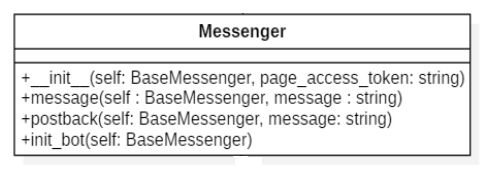
\includegraphics[width=\linewidth]{./pictures/class_messenger}}
\caption{Class Messenger}
\label{fig:class_messenger}
\end{figure}
\FloatBarrier

\subsubsection {Purpose}

The Facebook Messenger chatbot needs Facebook Messenger API to interact with the facebook users who need our service. This module can provides a connection with the Facebook Messenger API, so chatbot can send message to users and receive message from users through this module. It is the most important factor that allows the messenger to function.  

\subsubsection {Functionality}

This module makes chatbot be able to send messages to the users and receive messages from the users. There is a Facebook server between users and our chatbot server. Facebook provides a webhook function and it gives our chatbot server alerts that user sent a message to our chatbot or other user reaction to our chatbot (entering chatbot chatroom etc.) and messages. Through this module, we can give a response to users immediately and can provide our service. When users send messages, we can implement the appropriate chatbot action and build scenarios in which to communicate with users. It also provides the transmission of text as well as other extension files, such as pictures and files, to enable context-sensitive types of messages to be sent. 

\subsubsection {Location of Source Code}

/project/src


\subsubsection {Class component}

The messenger module has messenger class. It extends BaseMessenger class, that is provided from the fbmessenger package. fbmessenger is a python library to communicate with the Facebook Messenger API's. It provides various functionality and class to implement the chatbot service. The class doesnt have a variable and it has serveral methods for service. The methods that class has are as follows:

\begin{itemize}
\item \_\_init\_\_(self:BaseMessenger, page\_access\_token): constructor of the messenger class. it makes messegner object.
\item message(self: BaseMessenger, message): The message function is called when we get a "message" object from the webhook. The webhook can send a few different json messages, and we can specify which message types we want to receive when we set up the webhook. And message() is general when the user sends us a message. So in the message function, when we receive a message we first send an achknowledgment to the user that we received it and computing it. 
\item postback(self: BaseMessenger, message): This method can handle a postback webhook. The Facebook Messenger supports the postback meun for users. The users can invoke an action in our bot through the button. When users press the button to invoke some actions in cahtbot, chatbot receives a postback webhook from the Facebook Messenger server. This function can handle this webhook, so can give some responses to the user.
\item init\_bot(self: BaseMessenger): the init\_bot method initiate our chatbot. It initiate greetings and actions list that the users can select when they start our chatbot. And, it also provides customized buttons function that the users can choose during the scenario. 
\end{itemize} 

\FloatBarrier

\subsection{Module 2 - fb\_bot}


\begin{figure}[htbp]
\centerline{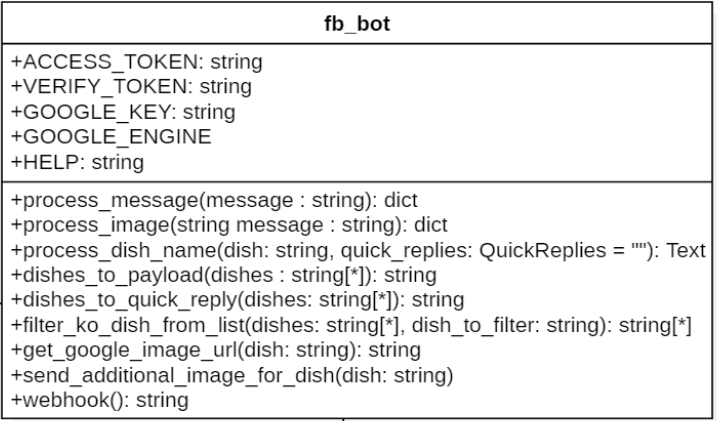
\includegraphics[width=\linewidth]{./pictures/class_fb_bot}}
\caption{Class fb\_bot}
\label{fig:class_fb_bot}
\end{figure}
\FloatBarrier


\subsubsection {Purpose}

We need an intermediary between our chatbot and functionality of our service. A module fb\_bot plays such a role. The module fb\_bot allows each module to be grouped and became a bridge that enables our services to be delivered to users.


\subsubsection {Functionality}

The fb\_bot module handles messages from the module messenger to reply to users. When the messenger gets text from the users, the module processes a message in condition of the text. If a messenger gets a picture type file from the users, the module fb\_bot calls a module analyzer to analyze picture that gets from user and get information of dishes from our database. And It process our data that is from module analyzer agian, and sends back to the module messenger to give results to the users. The module fb\_bot has several functionalties to interact with other modules.


\subsubsection {Location of Source Code}

/project/src


\subsubsection {Class component}

The class fb\_bot has three member variables. They are as follows:

\begin{itemize}
\item ACCESS\_TOKEN:string : ACCESS\_TOKEN is for accessing to the the chatbot messenger. Each chatbot has an unique ACCESS\_TOKEN. A module fb\_bot can get messages from the bot using the token. We need it everytime we send a message to facebook. 
\item VERIFY\_TOKEN:string : it is used when facebook senta a first message to check if the server exists. the VERIFY\_TOKEN can be anything we want to, we just have to specify it when setting up the webhook.
\item HELP:string : When user write 'help' or type some messages that is not related to request for our service, chatbot sents this string.
\end{itemize} 

The methods that class fb\_bot has are as follows:

\begin{itemize}
\item process\_message(message):dict : This method returns reply message based on the type of message sent by the user. There are several conditions in it, and it retuns specific reply that the user wants. It can be the scenario handler for our chatbot. I can handle all kinds of type of messages.
\item process\_image(message):dict : This method is only for the condition when user send picture type message that users want to know about. It calls analyzer method to get an infromation of dishes and returns description about dishes. It includes all the action messages while the picture analyzes and the information receives. In the action messages, the quick reply type message is included in here. 
\item dishes\_to\_payload(dishes, current\_dish):string : The method is used in the dishes\_to\_quick\_reply method. It saves dish list as a jason format.
\item dishes\_to\_quick\_reply(dishes, current\_dish):string : The method is for replying to quick reply message type. A quick reply message is one of the message type that Facebook Messenger supports, it consists of the button list. When the fb\_bot module gets dish list from the analyzer module, it creates the quick reply buttons for user to choose one of them to get a information. It calls dishes\_to\_payload method to save the list of dishes that it havent given yet to the users.
\item webhook():string : The webhook method controls the connection between Facebook Messeneger server and the chatbot server. It uses Flask, the microframework for python. It uses VERIFY\_TOKEN to check if the server exists. And if it exists, It initiates our chatbot service using init\_bot method in messenger module.
\end{itemize} 

\FloatBarrier


\subsection{Module 3 - analyzer}



\begin{figure}[htbp]
\centerline{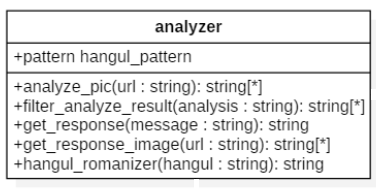
\includegraphics[width=\linewidth]{./pictures/class_analyzer}}
\caption{Class Analyzer}
\label{fig:class_analyzer}
\end{figure}
\FloatBarrier

\subsubsection {Purpose}

A module analyzer has an important role in our service. We need to extract korean letters from the picture, and find the dish names about which users want to know. Therefore, this module is necessary to analyze image. It linked with our main service function, Azure OCR Text Recognition API. And, it makes requests to get analysis results from it. It also serves final information that user wants. 

\subsubsection {Functionality}

The module analyzer processes image through the OCR Text Recongnition API to extract the text from the image. When it gets result from Recognition API, it searchs only krorean letters from the result. It becomes a list of the dishes that users want to know. Then analyzer sends a query to the db module to search description for that dish name. It also romanizes korean dish name to roman and provides the name with description to the fb\_bot.

\subsubsection {Location of Source Code}
/project/src

\subsubsection {Class component}


\begin{itemize}

\item pattern hangul\_pattern : The pattern is used to distinguish whether the text is hangul or not.
\item analyze\_pic(url):string[*] : The analyze\_pic() method checks the image url that comes from users is available, and sends request to the Azure OCR Text Recognition API. It needs specific json type input, so it organizes the format and returns result that is from the API.
\item filter\_analyze\_result(analysis):string[*] : The method filter analyze result() gets analysis as a parameter. This the return value of analyze\_pic() method. When it called, the method extracts only korean letters from the analysis string list. The pattern hangul\_pattern is used to distinguish korean letters from the list. 
\item get\_response(message):string : A get\_response method is called when user sends dish name. It calls db module to get information of dish from database server, and it combines dishe's korean name, its roman name and description. When it creates final description, it returns the description.
\item get\_response\_image(url):string[*] : The method is called when user sends picture of menu. It calls filter\_analyze\_result method to get the korean dishes list and it sends query to find information from the server. and it returns the description of dish.
\item hangul\_romanizer(hangul):string : The hangul romanizer method romanize dish name. it uses python library hangul\_romanize. It support Tarnsliter class and it just makes korean text to roman. 
\end{itemize} 

\FloatBarrier

\subsection{Module 4 - db}

\begin{figure}[htbp]
\centerline{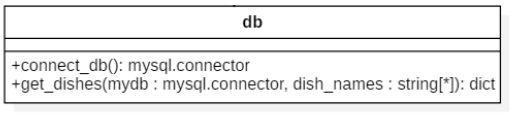
\includegraphics[width=\linewidth]{./pictures/class_db}}
\caption{Class db}
\label{fig:class_db}
\end{figure}
\FloatBarrier

\subsubsection {Purpose}

The module db is used to get information of dishes from the database server.   
\subsubsection {Functionality}

We have own MySQL database that stores description of the dishes. The module makes a connection with the MySQL database server and it can send queries to the database server and get a result of the query. 


\subsubsection {Location of Source Code}

/project/src

\subsubsection {Class component}

The class has no member variable, and the class methods are as follows:

\begin{itemize}
\item connect\_db():mysql.connector :  It makes a connector object to connect with our MySQL server to send the query to it. It includes the connection information to connect to database. It uses mysql.connector library to get the mysql.connector class. 

\item get\_dishes(mydb, dish\_names):dict : It sends a query for getting dishes information to the database server using the connector object. The query is for getting descriptions of specific dish name that the module analyzer gives as a parameter. And it returns the results from the database as dictionary. \newline
\end{itemize}

\FloatBarrier

\begin{figure}[htbp]
\centerline{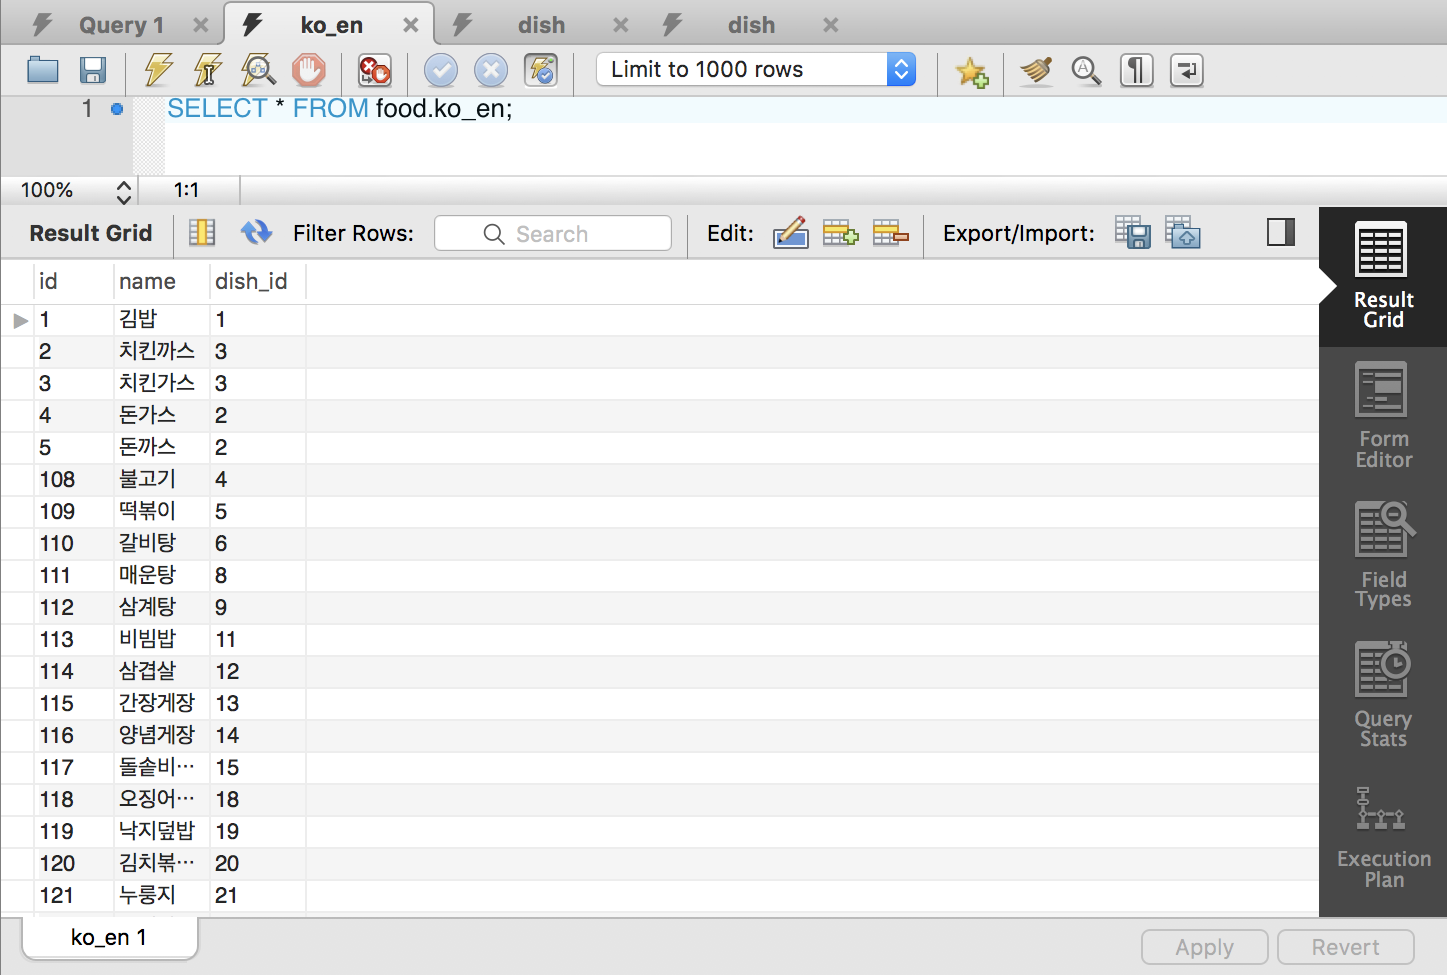
\includegraphics[width=\linewidth]{./pictures/database_ko_eng}}
\caption{Matching dish names from Korean to English}
\label{fig:Matching dish names from Korean to English}
\end{figure}
\FloatBarrier
Database for translation from Korean to English.

\begin{figure}[htbp]
\centerline{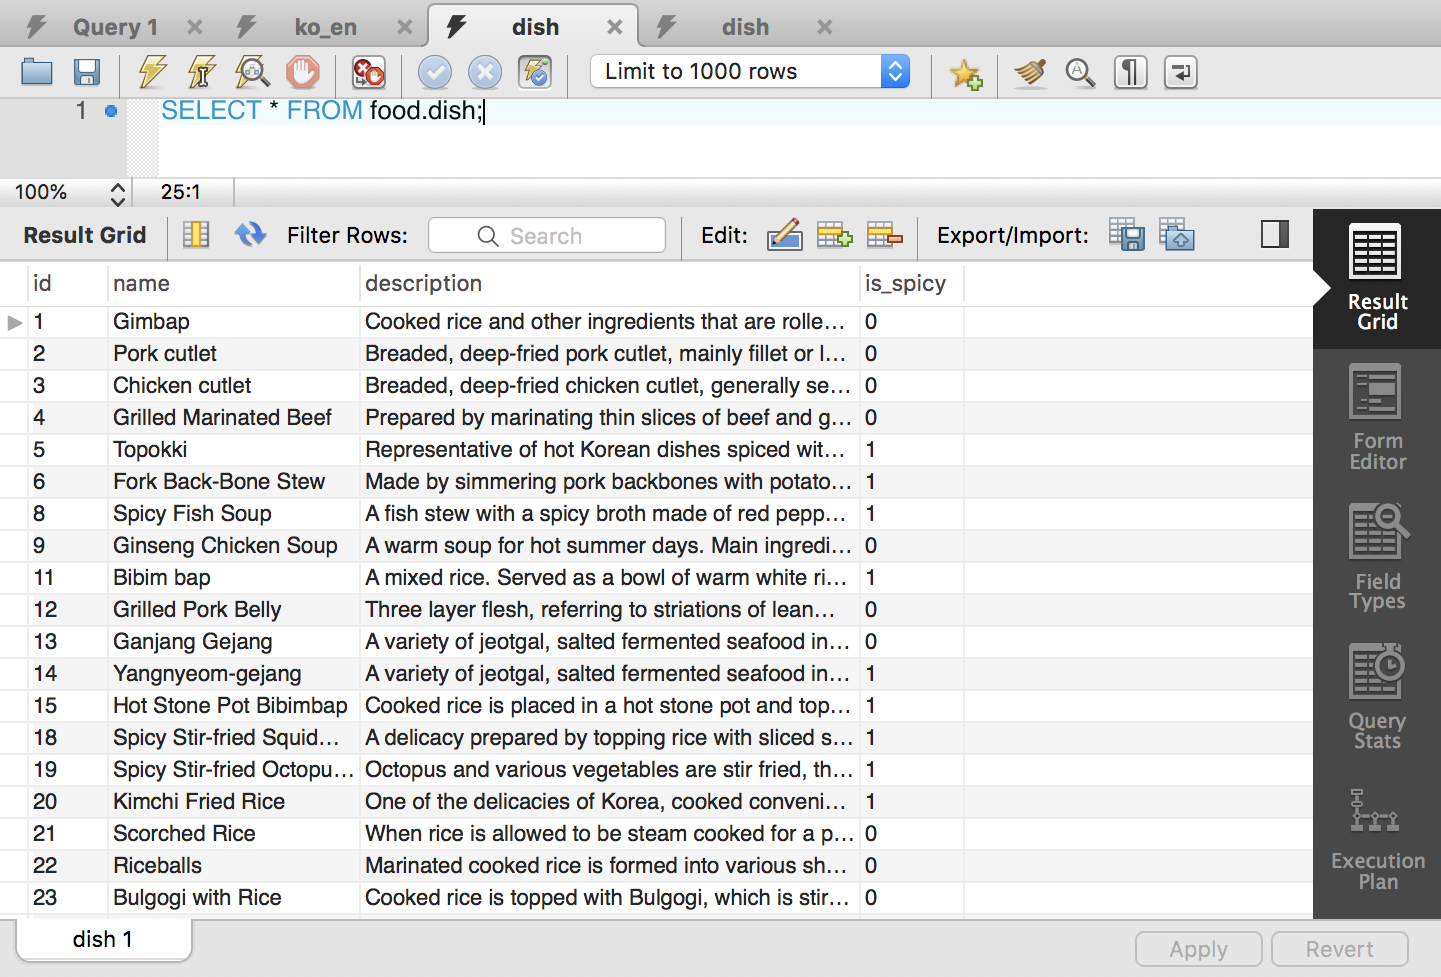
\includegraphics[width=\linewidth]{./pictures/database_dish_list}}
\caption{Example of dish list in database}
\label{fig:Example of dish list in database}
\end{figure}
\FloatBarrier
Database for food name and description in MySQL Workbench.\newline\newline


\section{use cases}

\subsection{Chatbot platform}
We decided to build chatbot through Facebook, which has more than 2 billion users until 2017. Facebook Messenger can provide an intensively tested and user-friendly interface because many people are already using it. In addition, users who are using Facebook do not require a separate download, so we can meet Requirements A4.

\subsection{Description of practical usage}

\begin{figure}[htbp]
\centerline{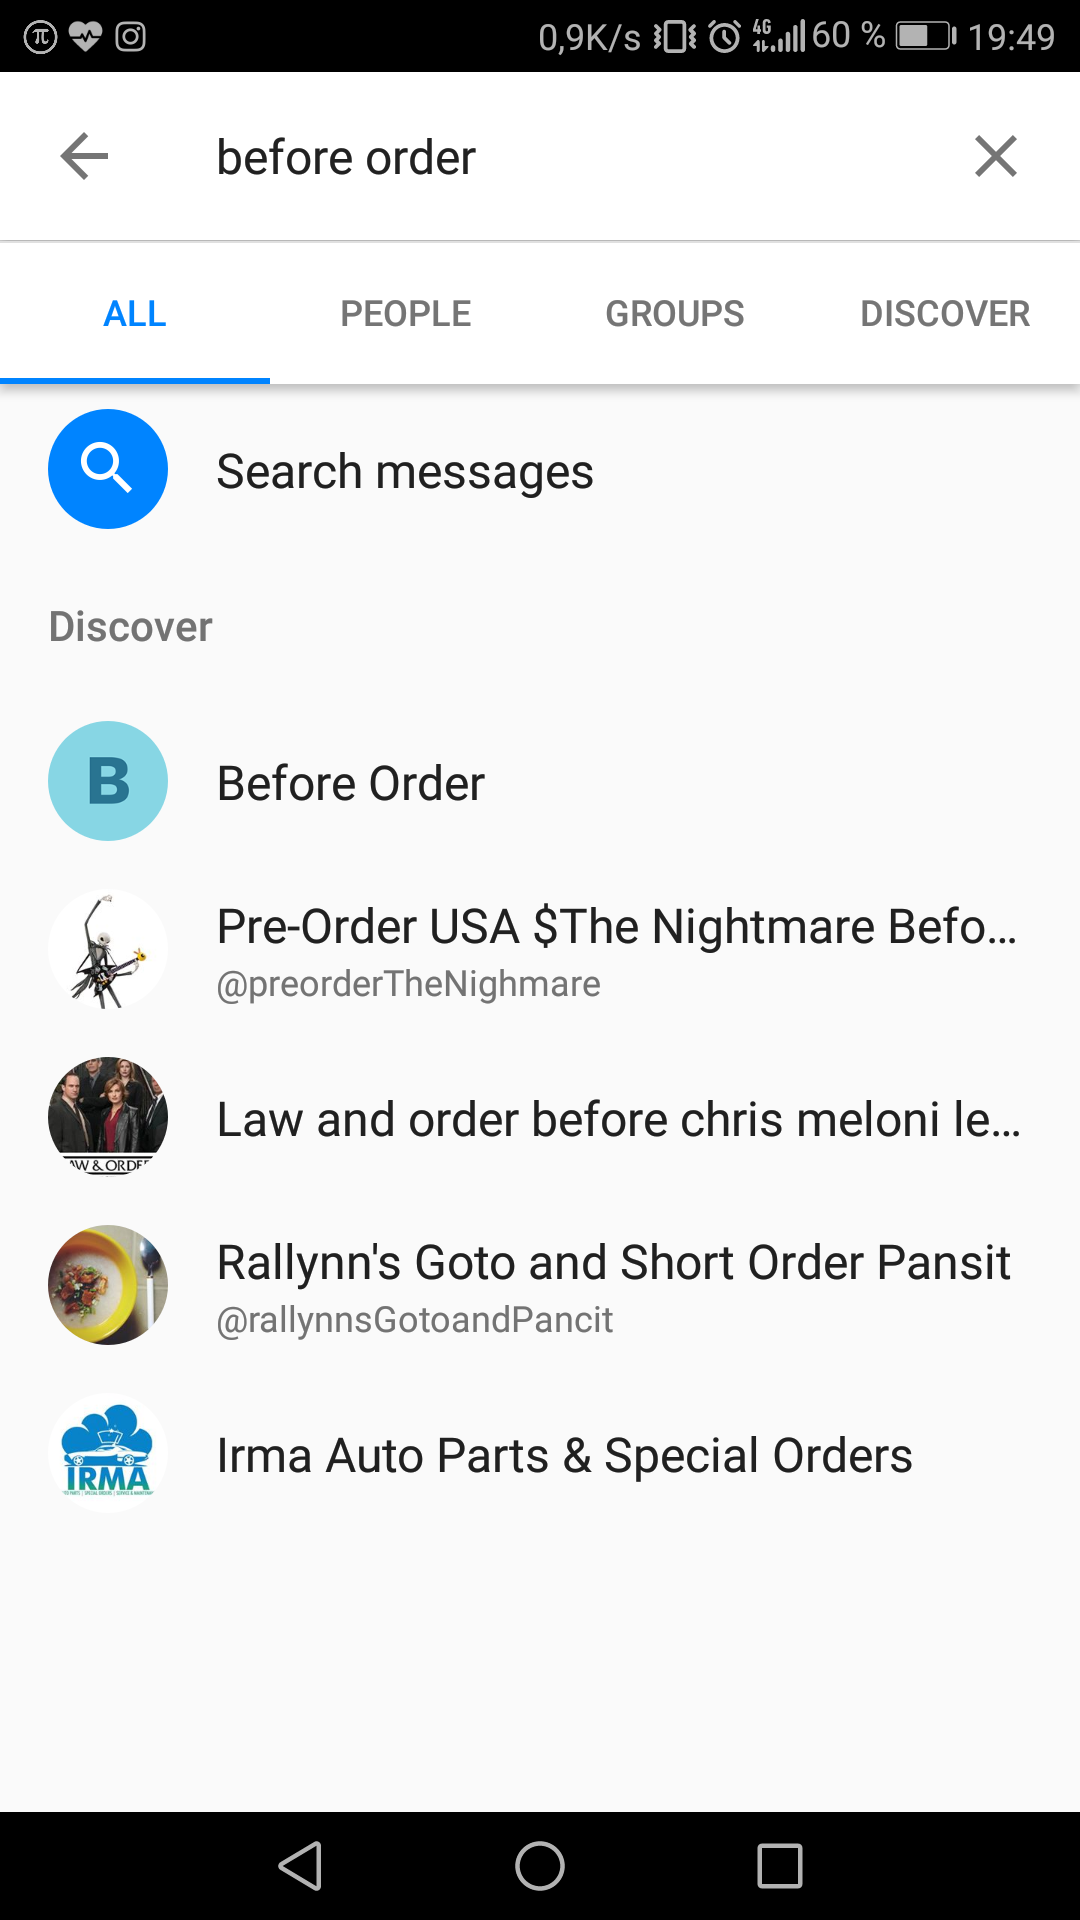
\includegraphics[height=\custompicheight]{./pictures/Screenshot_20181125-194915}}
\caption{Search \emph{Before Order} in Facebook Messenger}
\label{fig:Before Order_search}
\end{figure}
\FloatBarrier
\subsubsection{Search Before Order}
Access Facebook Messenger through a variety of devices. Then users should search our chatbot ‘Before Order’ in Facebook Messenger. As seen from the above capture, ‘Before Order’ is available on smartphone and therefore this meets the requirement A.1.

\begin{figure}[htbp]
\centerline{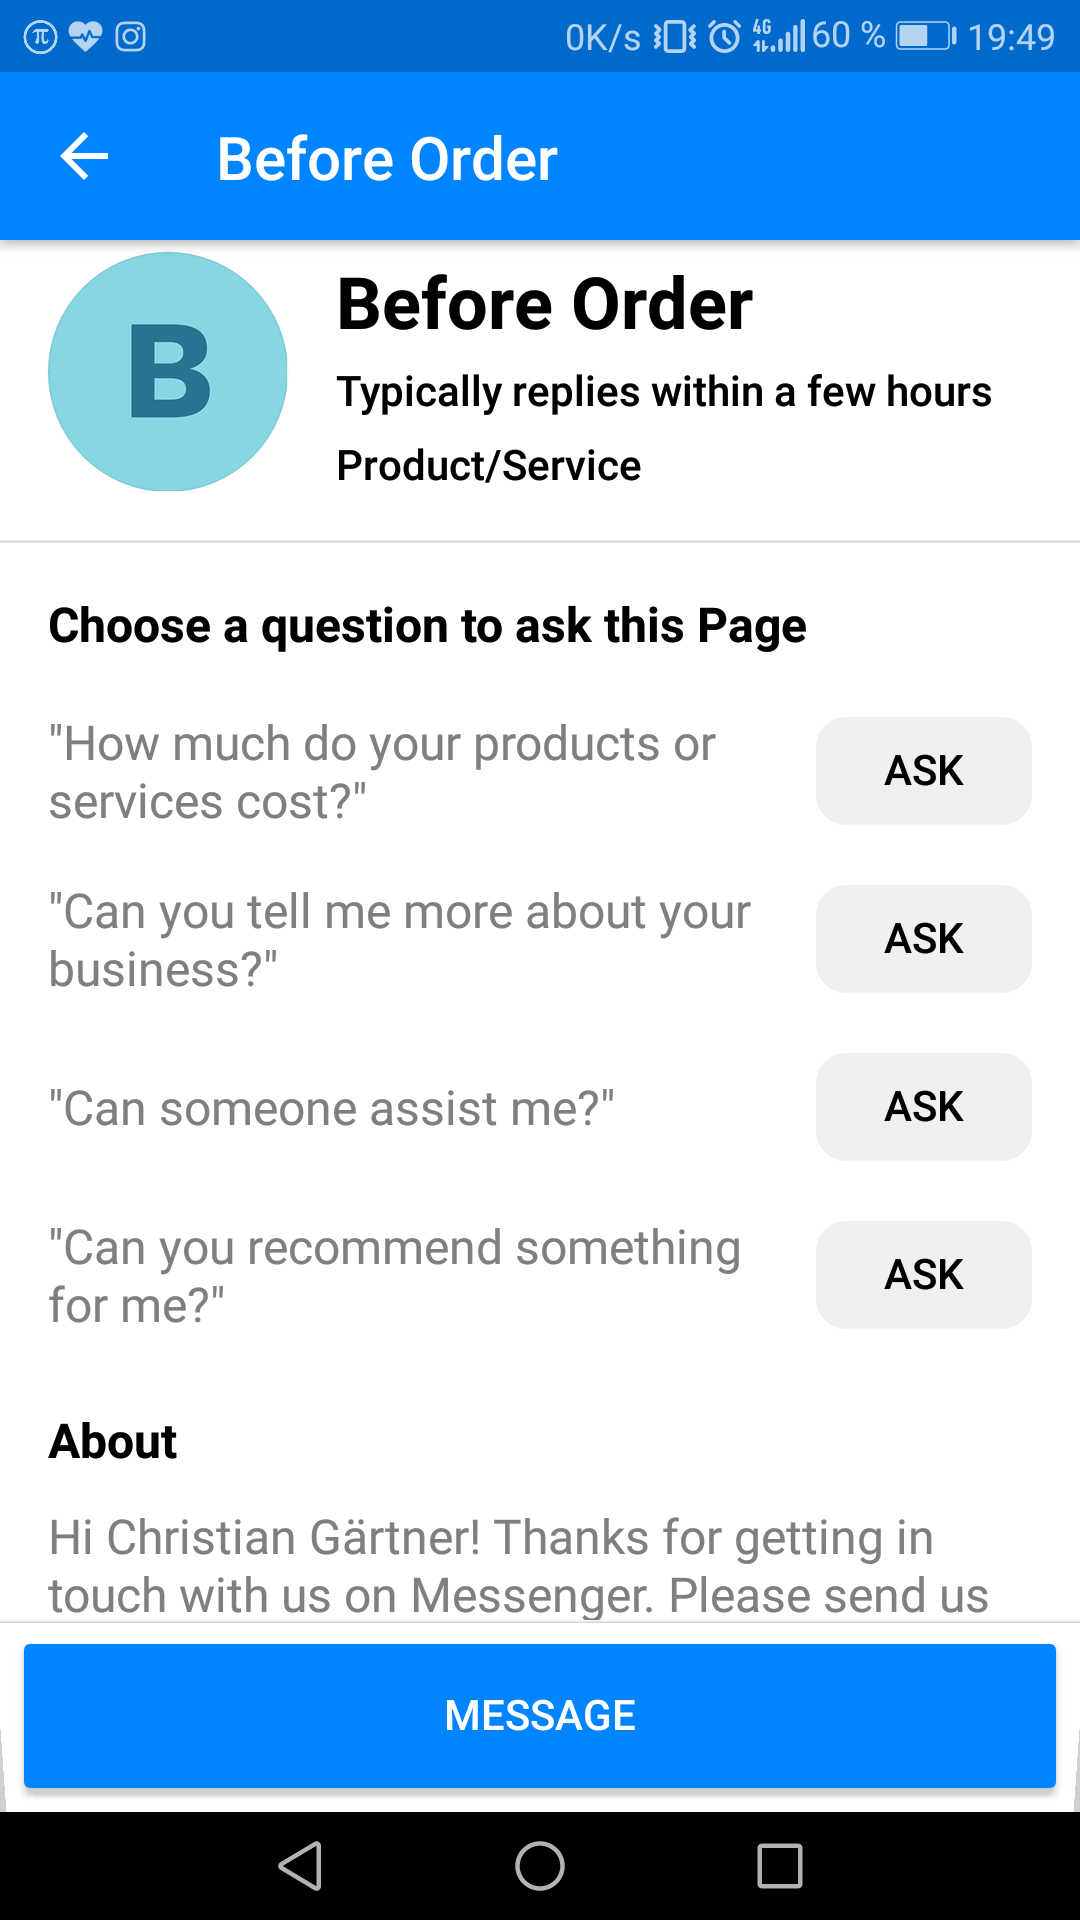
\includegraphics[height=\custompicheight]{./pictures/Screenshot_20181125-194938}}
\caption{Initial screen page of \emph{Before Order}}
\label{fig:Before Order_initial_screen}
\end{figure}
\FloatBarrier
\subsubsection{Start messaging}
 If users find ‘Before Order’, they can click it and start Messenger chatting. Click the button ‘Message’ or ‘시작하기’ in order to send messages to chatbot. By using existing Facebook Messenger, ‘Before Order’ is easily accessible to billions of people using Facebook and its Messenger. Users even do not need to newly sign up for ‘Before Order’.


\begin{figure}[htbp]
\centerline{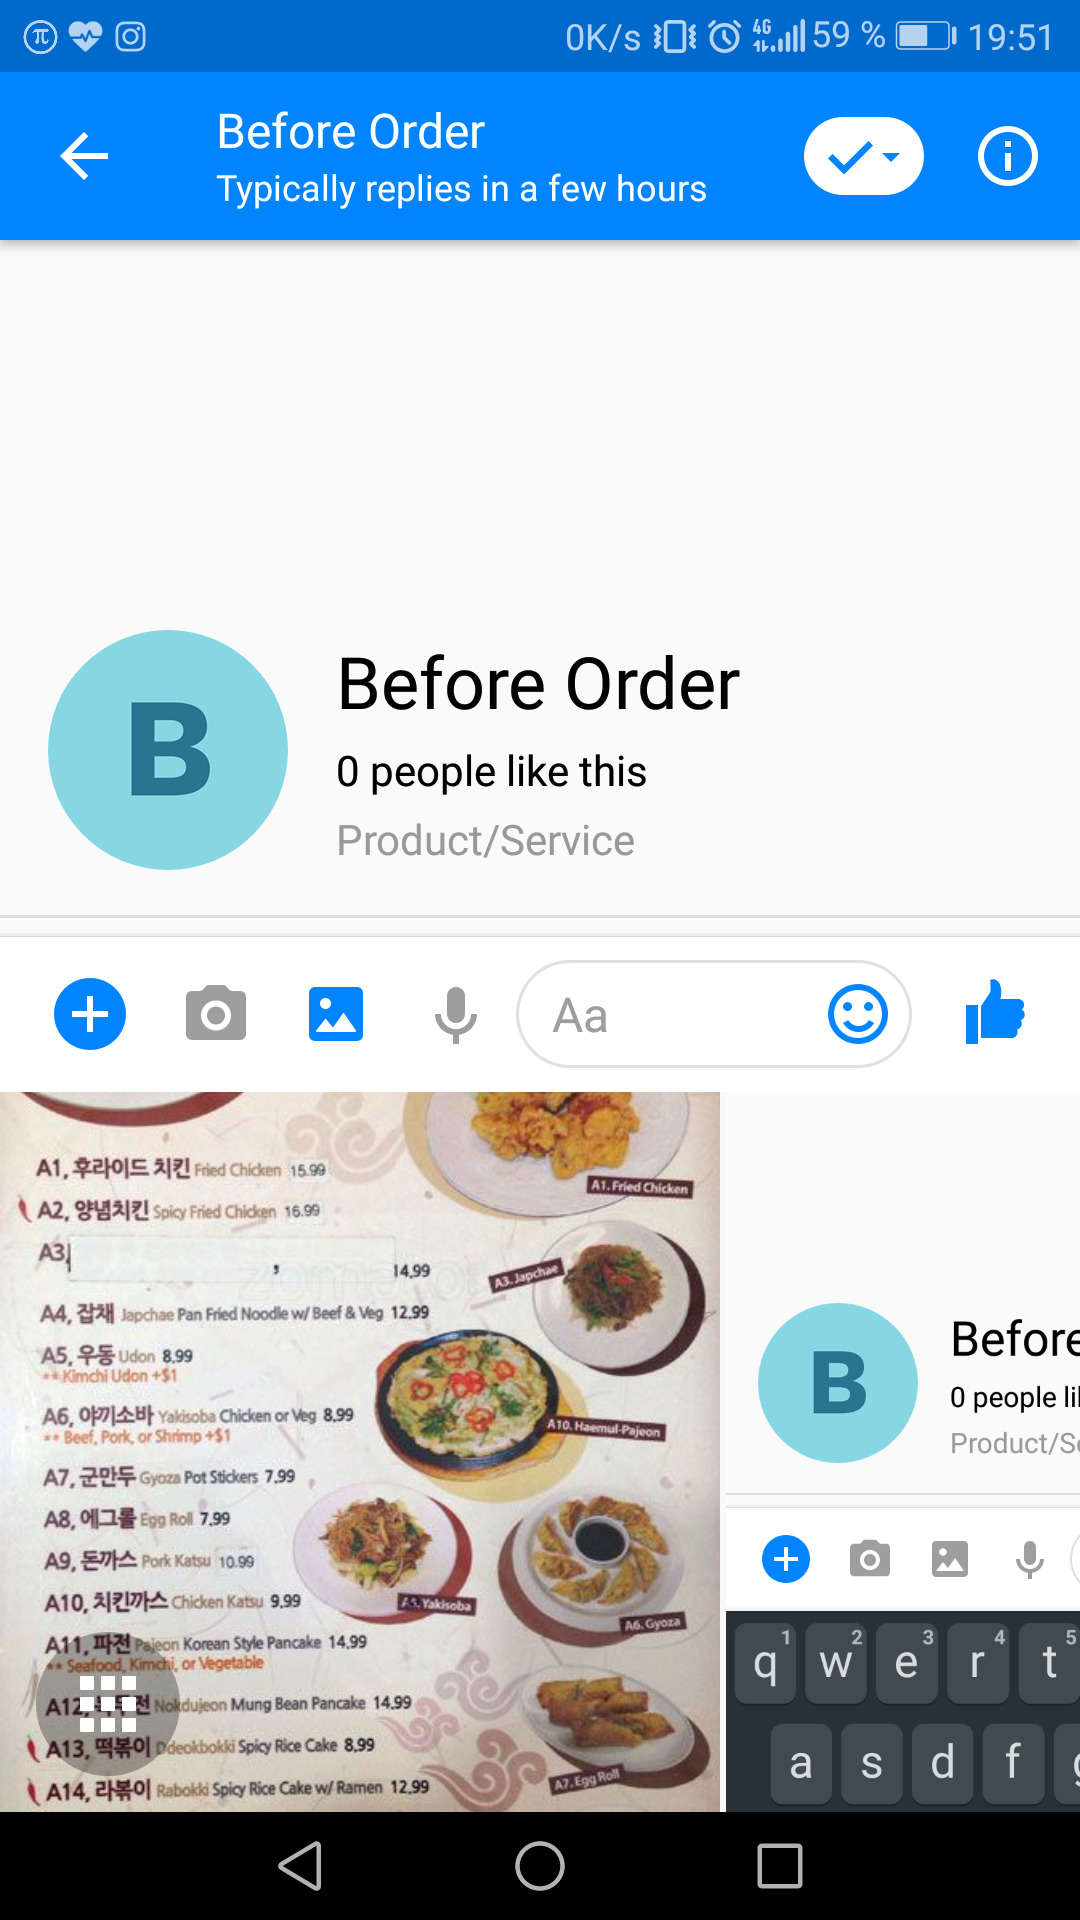
\includegraphics[height=\custompicheight]{./pictures/Screenshot_20181125-195124}}
\caption{Selecting menu picture as an input}
\label{fig:Before Order_input_selection}
\end{figure}
\FloatBarrier
\subsubsection{Select input}
 If users entered ‘Before Order’ page, the chatbot will deliver a brief greeting. Our chatbot was made for foreigners who had trouble translating the Korean menu. Therefore ‘Before Order’ take optimized way of relieving their inconvenience. Whenever users find it difficult to interpret the Korean menu in a restaurant, they can just take a picture of the menu and then select the picture to send.


\begin{figure}[htbp]
\centerline{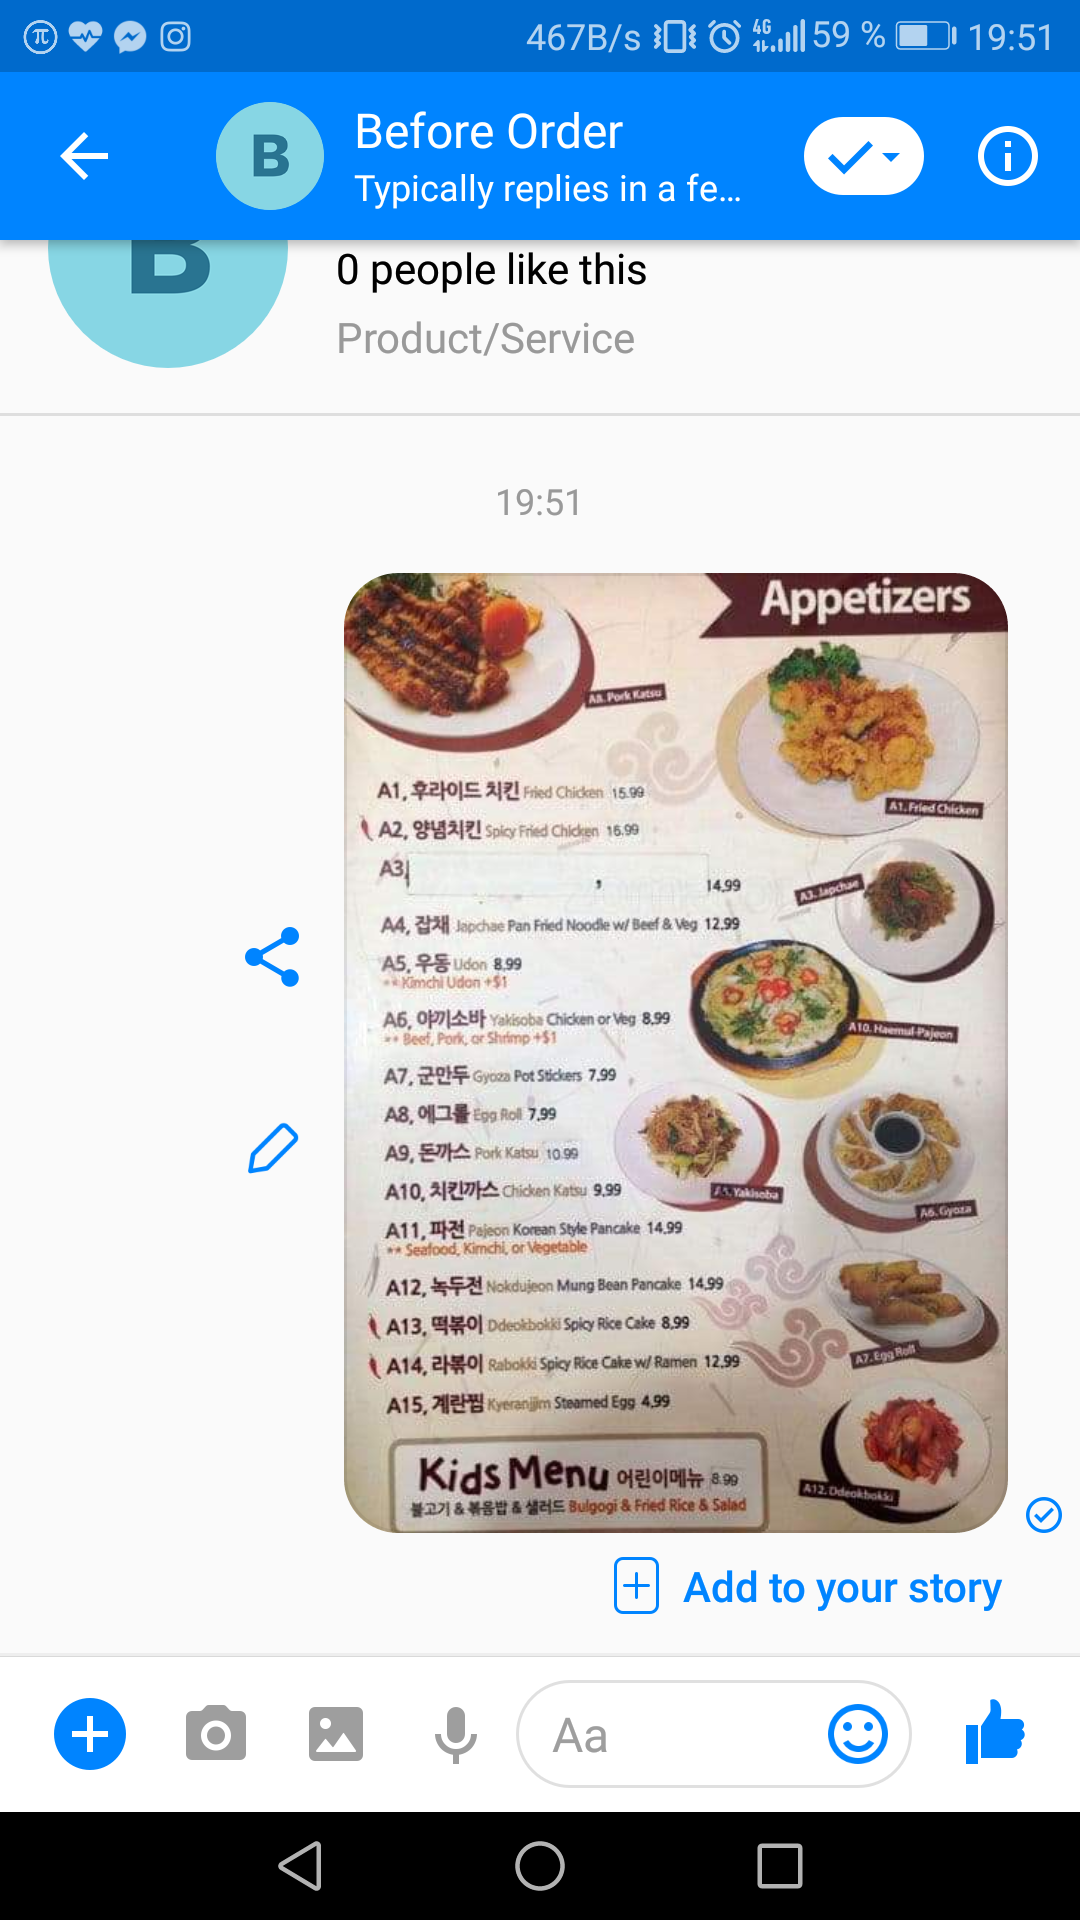
\includegraphics[height=\custompicheight]{./pictures/Screenshot_20181125-195145}}
\caption{Users sending input to \emph{Before Order}}
\label{fig:Before Order_send_Input}
\end{figure}
\FloatBarrier
\subsubsection{Send input}
The users who are not familiar with Korean menus can get the information they want through 'before order'. Users take a picture of the menu using the camera on the device you are carrying. Using Facebook Messenger, the users can send a message through camera or photo button in the lower left corner. Then send 'before order' and we will begin to recognize the menu.


\begin{figure}[htbp]
\centerline{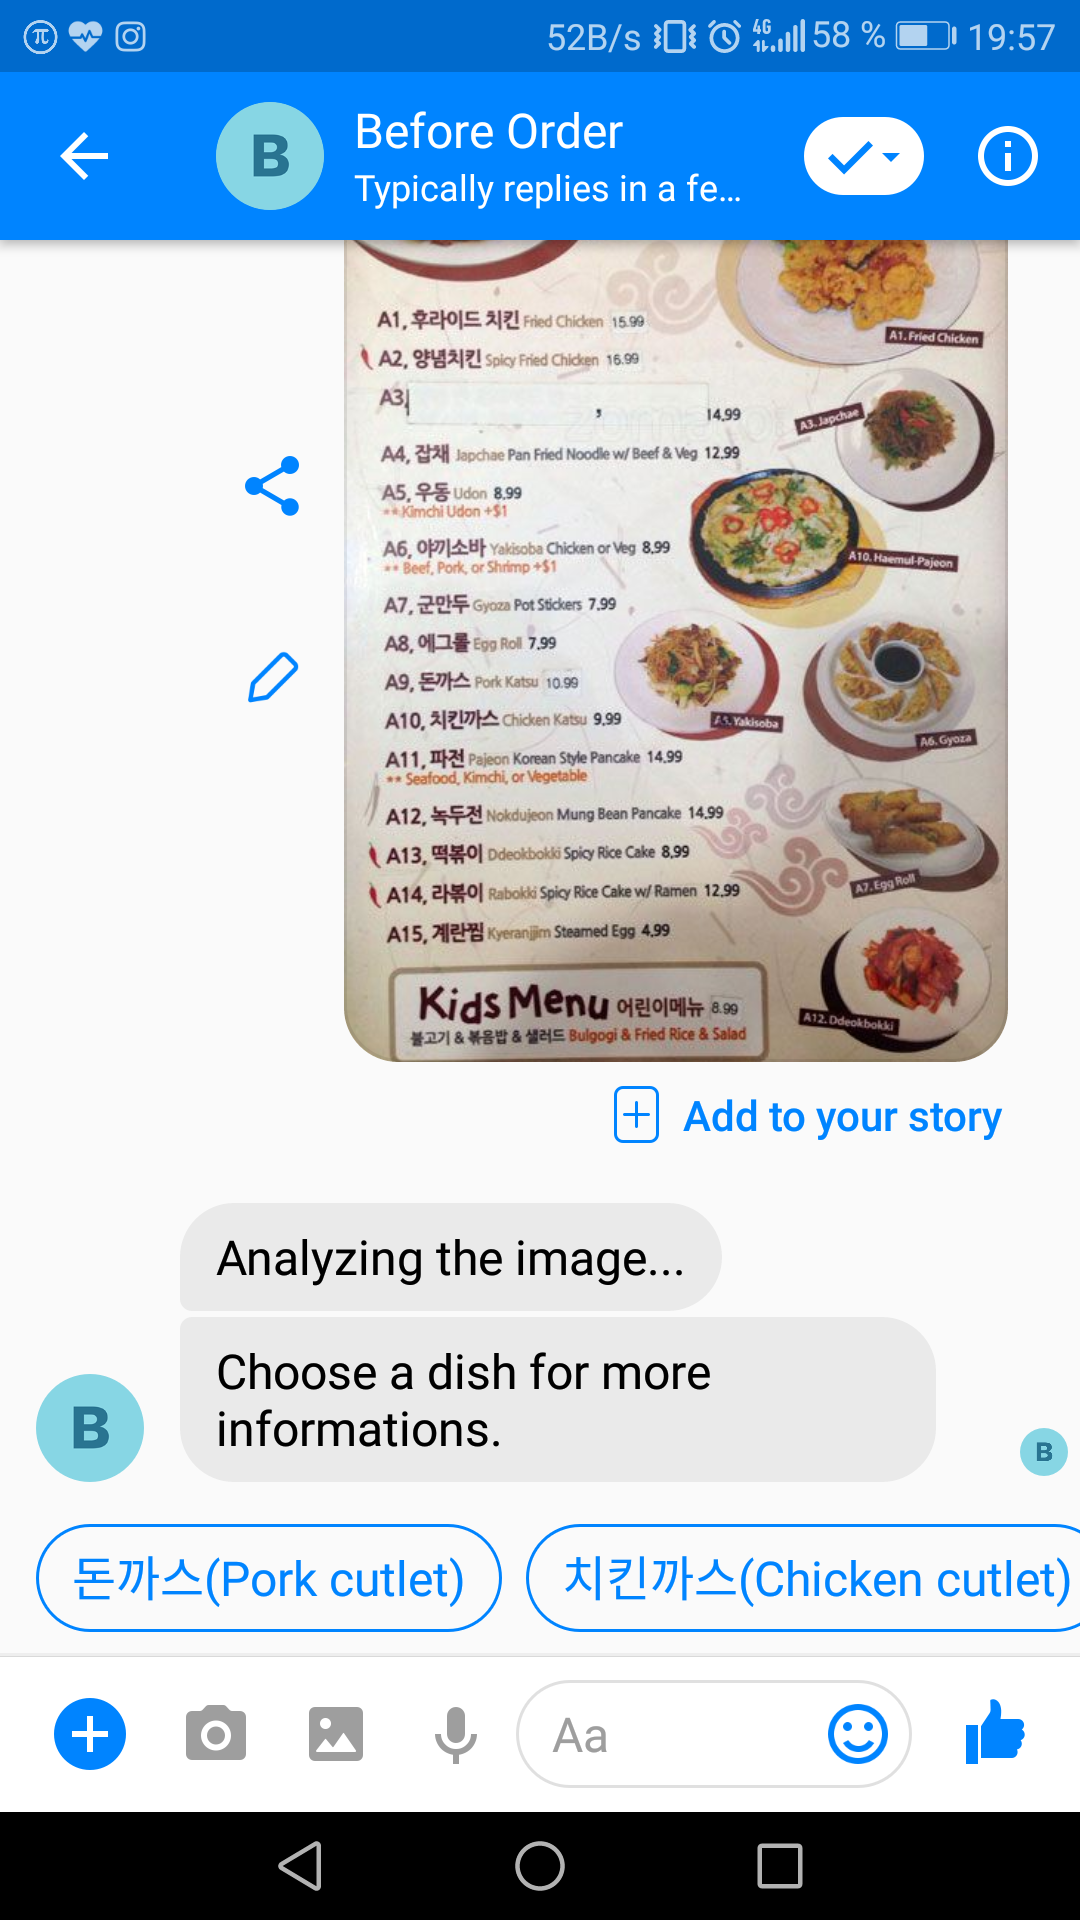
\includegraphics[height=\custompicheight]{./pictures/Screenshot_20181125-195722}}
\caption{Analyzing the input sent from user}
\label{fig:Before Order_analyze_input}
\end{figure}
\FloatBarrier
\subsubsection{Wait for the result}
 Based on the pictures sent by the user, we will begin to analyze the images. Users can view the message 'Analyzing the image' while the image is being analyzed and may be asked to select the desired information after the analysis is completed. Users can click on a list of buttons that are created based on the text we recognize.


\begin{figure}[htbp]
\centerline{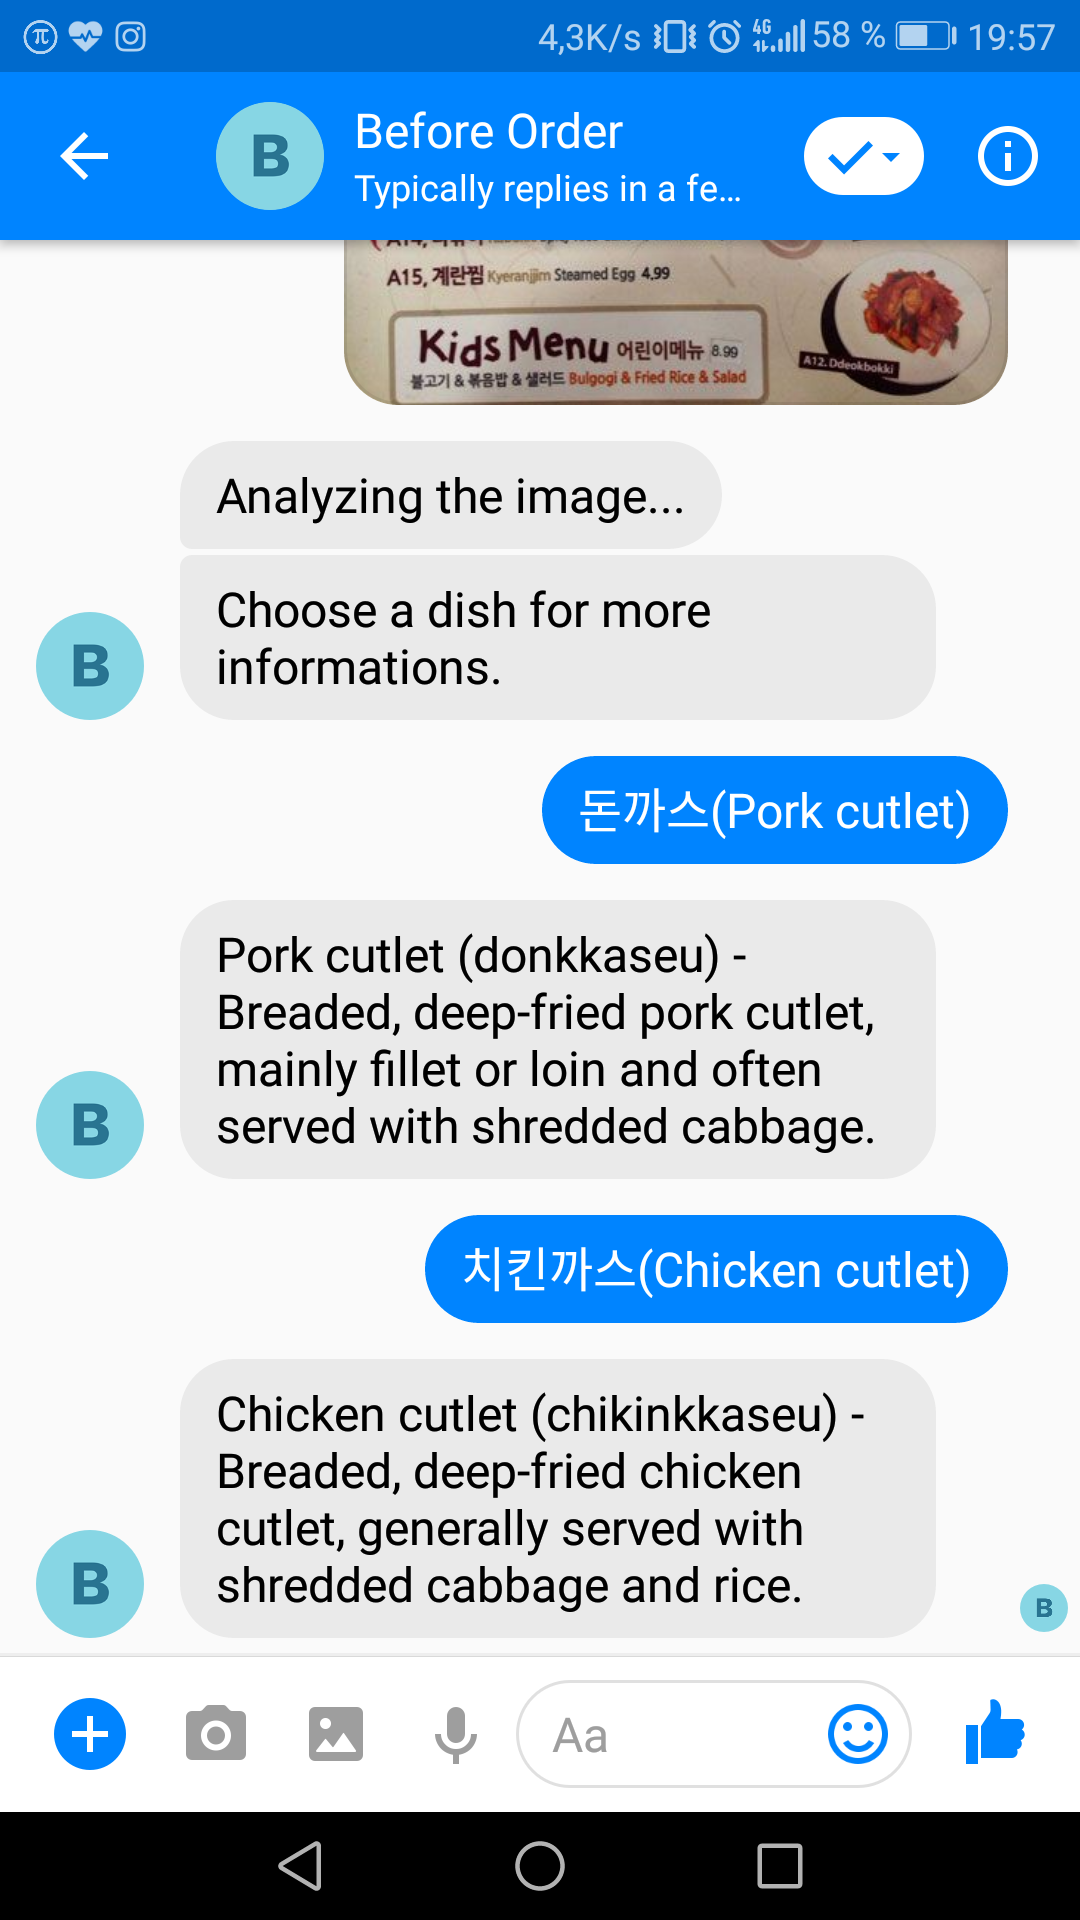
\includegraphics[height=\custompicheight]{./pictures/Screenshot_20181125-195753}}
\caption{Showing information about the selected dish}
\label{fig:Before Order_show_dish information}
\end{figure}
\FloatBarrier
\subsubsection{Receive a selected dish information}
When users click the button with dish name, dish information appears in the way as the picture above. As stated in the requirement A.8, All information is provided in English except for user input. As a result of chatting with ‘Before Order’, users get a brief description of the dish and information about its ingredients. This is a key feature of ‘Before Order’ which satisfied the requirement A.9. To provide information from the database with such reliability, one more thing – price value should be taken into consideration. Though dish name ‘치킨가스’ is displayed along with the price value 9.99 in the given menu picture, ‘Before Order’ succeeded in recognizing only the dish name by adding the function of excluding the price portion. These features make it possible to retrieve the right information from the database and therefore meet the requirement A.12. To follow the requirement A.13, all the dish information was taken form Wikipedia and this guarantee both accuracy and reliability. Small but important feature is the Romanization. Inside the parentheses, there is Korean dish name written in Roman characters like ‘donkkaseu’ and ‘chikinkkaseu’. By referring to the Romanization, users can well pronounce Korean dish name in the case of ordering food .This function is implemented to meet second condition inside the requirement A.13.


\subsection{Addressing error-prone cases}

\begin{figure}[htbp]
\centerline{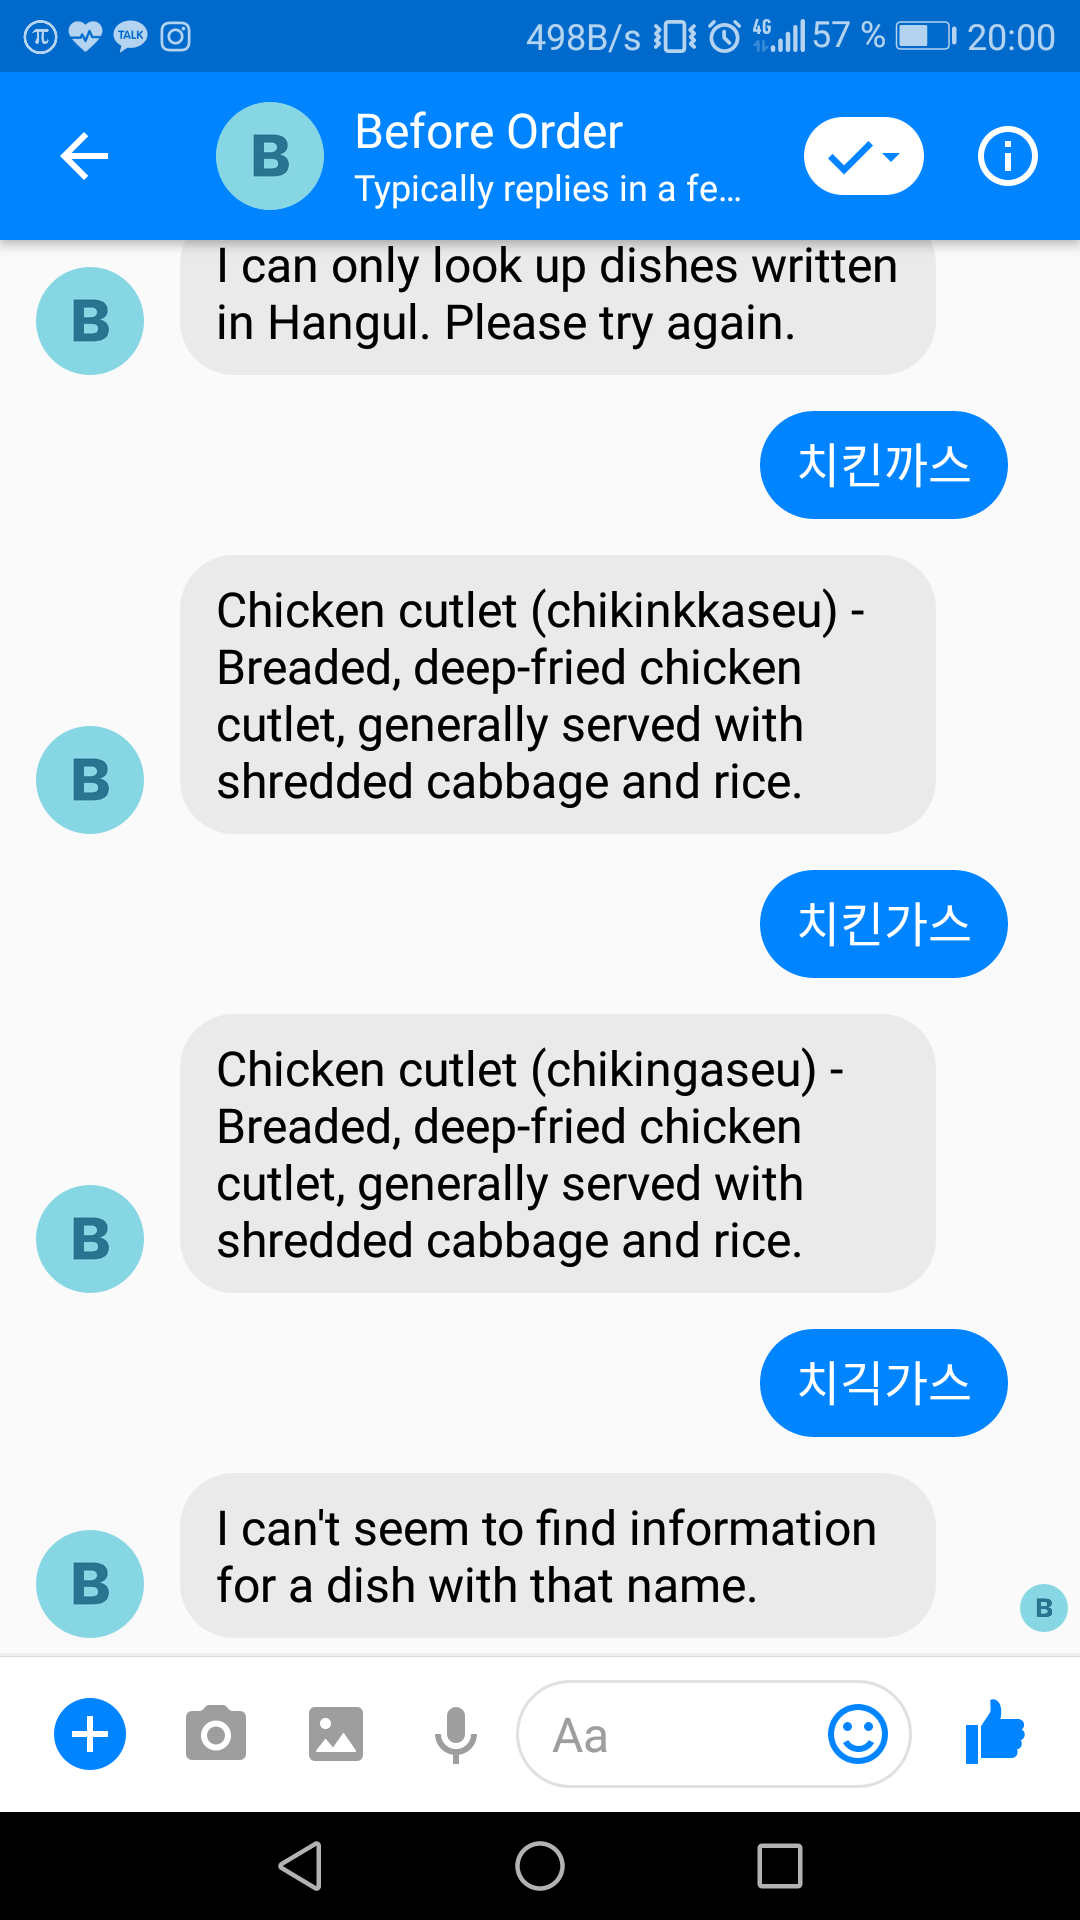
\includegraphics[height=\custompicheight]{./pictures/Screenshot_20181125-200020}}
\caption{Handling various error-prone cases}
\label{fig:Before Order_features}
\end{figure}
\FloatBarrier
The basic function set of ‘Before Order’ is to receive photos sent by users, analyze them, and provide a list of buttons. However as stated in the requirement A.7 and A.10, our chatbot ‘Before Order’ can recognize not only pictures but also Korean inputs – food written in Korean sent by users. Even if the user enters Korean words ‘치킨까스’ or ‘치킨가스’ without menu pictures, It is also able to provide accurate food information. This satisfies the third item of requirement A.13. Furthermore ‘Before Order’ is designed to support various expressions of Hangul. It successfully recognize two different expressions ‘치킨까스’ and ‘치킨가스’ as the same word. At the same time, ‘Before Order’ can also distinguish between dish names and random letter clusters. For random letter clusters like ‘치긱가스’, the chatbot send a response ‘I can’t seem to find the information for a dish with that name.’ - notifying something is wrong. This meets the requirement A.11.

\subsection{Cope wiith data shortage problems}

\begin{figure}[htbp]
\centerline{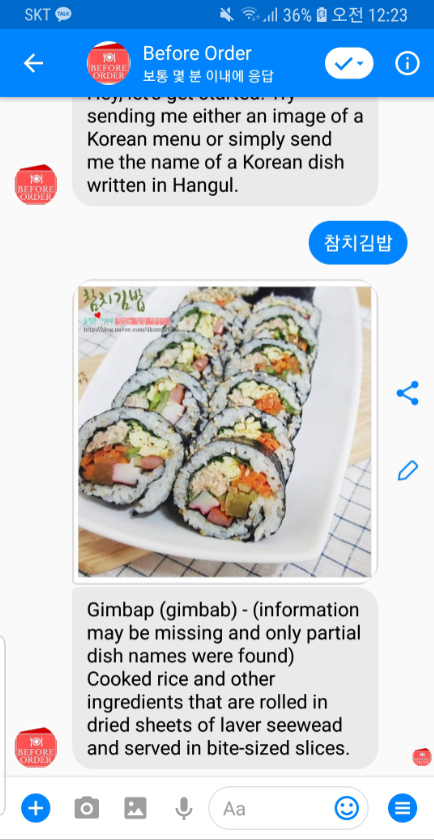
\includegraphics[height=\custompicheight]{./pictures/facebook_additional_feature}}
\caption{Cope wiith data shortage problems}
\label{fig:Before Order_features}
\end{figure}
\FloatBarrier

In cases where it is difficult to provide information because the dish required by the user is not stored in the database, we instead provide information about the larger range of food to which it belongs. For example, if the ‘참치김밥' information is not present on the database, it provides a description of’ gimbap’. Since ‘tuna gimbab’is a subset of normal ‘gimbab’ and the focus of information that users want is on ‘gimbab’ rather than ‘tuna’ itself, it is very useful and complements our weakness such as lack of database information. These additional chat-bot features are part of requirement A.13's reliable data delivery.

\subsection{Handling inappropriate input format}

\begin{figure}[htbp]
\centerline{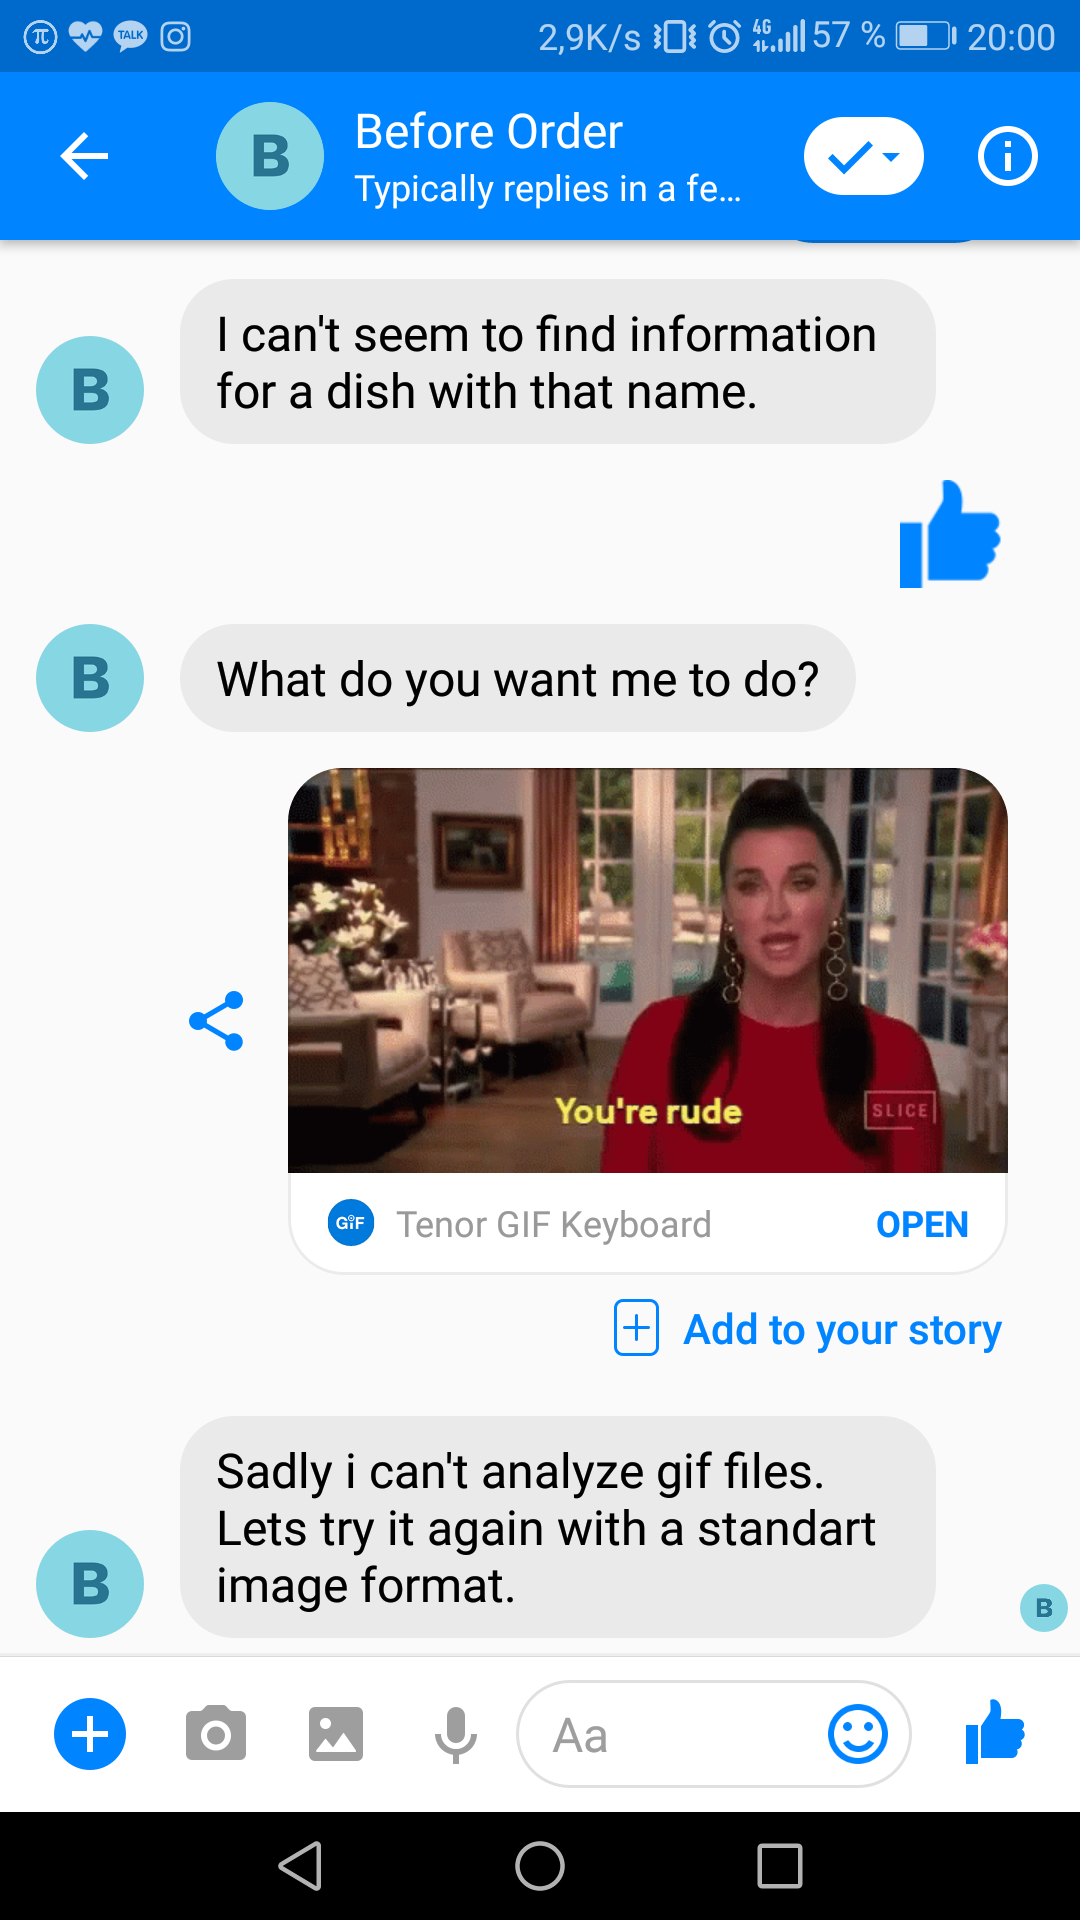
\includegraphics[height=\custompicheight]{./pictures/Screenshot_20181125-200053}}
\caption{Handling inappropriate image format}
\label{fig:Before Order_handling_error}
\end{figure}
\FloatBarrier

Just like the case of random letter clusters ‘치긱가스’, ‘Before Order’ can distinguish between right and wrong. If the user sends pictures in invalid format or pictures without a menu, the chatbot recognize them and give an appropriate response depending on the situation. This series of actions is designed to meet requirement A.11.


\subsection{Key functions}
As stated in Requirements A.6, we reduce the process of users searching menus in English and retrieving information about the word again. The users take pictures and send them to us without having to search again. Also, when users open the messenger window again, they can always see it again because they have a history of previous messages.

\subsection{Service management}
If the users are using the 'Before Order' and we cannot be aware of the message sent by the user, or if there is something we need to correct it, the users can contact us through the Facebook page. When a user posts a post on our page or sends an developer’s e-mail, we can provide feedback, like a requirement A5. And at the beginning of the conversation, we're specifying a message that we want users to send an email if they need help or if an error is detected...












\section{Discussion}

The Software Engineering course of the last three months have taught us all the importance of communication among team members and have been a valuable time to experience practical aspect of software implementation. But it is also true that there have been more difficulties than expected ever since we decided to implement the menu translation chat-bot, ‘Before Order’.

 First and foremost, the range of food that we had to provide was too wide. This was a problem because our team decided to build our own database and put dish information one by one. Because it was impossible to register tens of thousands of unique dish name in a team of four, the scope of information provided was reduced from nationwide to Wangsimni. That is, we’ve included all the foods of the common name (e.g. ramen) as a default, but had trouble including all the unique dishes or diverse expressions of the same dish at each restaurant (e.g. Aori ramen). Therefor it is part of our improvement task to keep up with menus and dish information that are constantly updated in restaurants. 

 In the beginning, we had a problem about delayed server response. This also was a big problem because chat-bot was meant to provide a quick response to the questions asked by users. Using the existing ngrok tool, we found that the network delay was caused by the long distance between the U.S and Korea when the Facebook server in U.S sends a webhook to our server in Korea. So to solve this problem, we created U.S located hosting server that can receive webhook by using Heroku. As a result the delay was significantly reduced because it enabled the communication within same country, U.S.

 Lastly apart form all these, there were matters to be considered In detail. For vision api issue, the text was not recognized when the picture quality was poor or there was a space between the names of the foods in the picture. The latter problem occurred because each letter written in space was recognized as a different word. Therefor we have changed the code so that dish names can be recognized not only in word units but also in line units.

 Even though we did not achieved everything as we planned, but we still achieved a lot of things. We are very grateful that we can have this kind of experience because it was an opportunity to learn teamwork and improve personally. \\


 github address: https://github.com/Akkarin1212/before\_order

\end{document}
